% TODO maybe introduce weaks and softs??

\chapter{Memory Management Fundamentals}

% Before getting into the details of how to implement your lifetime
% requirements,
The Java language has a \emph{managed runtime}. In part, this means that, as a
Java program runs, the Java runtime takes on the burden of key aspects of memory
allocation and reclamation. It is important to understand what Java does for
you, in forming its decision of when an object should be reclaimed, when
devising your lifetime management strategy. This level of management includes
automatic garbage collection of both instances and Java classes. Java has
feature that govern, on your behalf, important aspects of the lifetime of
objects. Unfortunately, these features often appear in the form of low-level JVM
hooks, or implicit behavior that you have to carefully govern, and so require
careful coding to make correct use of them. You need to appreciate what the
runtime is doing for you, before considering how to reshape object lifetimes to
better suit your needs.

\section{Managed Memory}
\index{Managed Memory}

A runtime that manages memory is one that takes care of memory allocation and
reclamation. Some memory is allocated on the \emph{stack}, and some, often as a
result of calls to {\tt new}, is allocated on various \emph{heaps}. Sometimes
the compiler takes care of reclaiming these memory allocations, and sometimes
there are background threads that take care of freeing up memory.

\paragraph{The Stack}
\index{The Stack}
Most languages come with a minimal form of built-in memory management, in the
form of the \emph{stack}. Each method invocation, in each thread, has memory
associated with it. For a thread, these areas of memory are pushed and popped,
as the thread invokes and returns from the execution of methods. The stack
memory that is set aside for a method invocation is commonly called a
\emph{stack frame}\index{stack frame}; historically, it has also been referred
to as an \emph{activation frame} or \emph{activation record}\index{activation
frame}\index{activation record}. In the case of the stack, it is the compiler
that manages the lifetime of each threads' stack frames. The compiler inserts
this stack management code, and so it is invisible to you except if you inspect
the generated assembly code.

In Java, as shown in
\autoref{fig:stack-frames}, each stack frame contains either primitive data or
pointers to memory that has been allocated as a result of calls to {\tt new}.

\begin{figure}
\centering
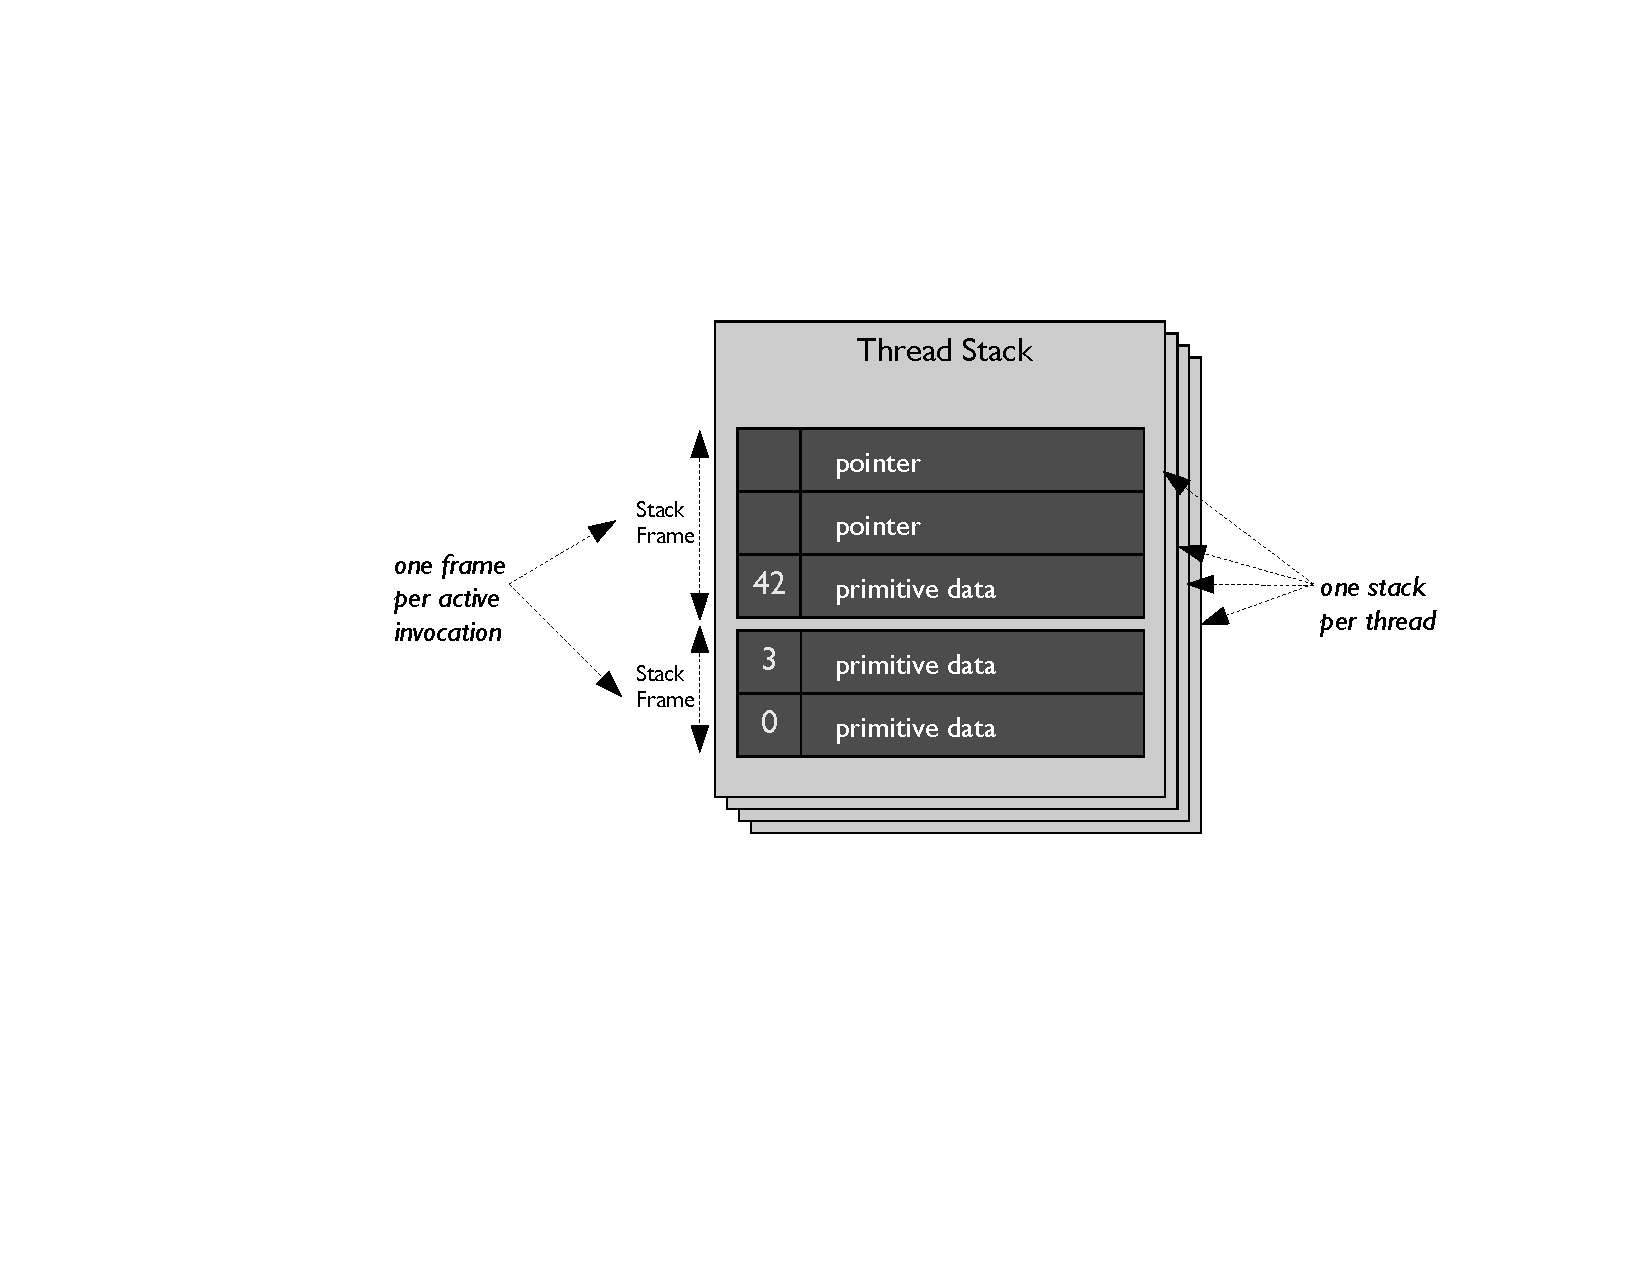
\includegraphics[width=0.8\textwidth]{part2/Figures/lifetime/heaps_and_stacks_stack_frames}
\caption{The compiler takes care managing the stack, by pushing and popping
the storage (stack frames) that hold your local variables and method
parameters.}
\label{fig:stack-frames}
\end{figure}

\paragraph{The Heap}

When you write Java code that allocates objects, the \jre a

%  a.b = new B();
%a.c = new C();
%a.b.d = new D();
%a.b.e = new E();
%a.b.e.f=new F();
  
\begin{figure}
\begin{subfloat}
\begin{minipage}[b]{0.4\textwidth}
\begin{shortlisting}
class B {
  D d;
  E e;
}
void foo() {
  A a = new A();
  G g = new G();
  ...
}
\end{shortlisting}
\end{minipage}
\caption{When coding in Java.}
\end{subfloat}
	\subfigure[When
	using
	Java,
	the stack can
	contain only primitive data and pointers to heap objects; each of those heap
	objects has a header that the \jre tacks on, for its own management
	purposes.]{\label{fig:heaps_and_stacks_java}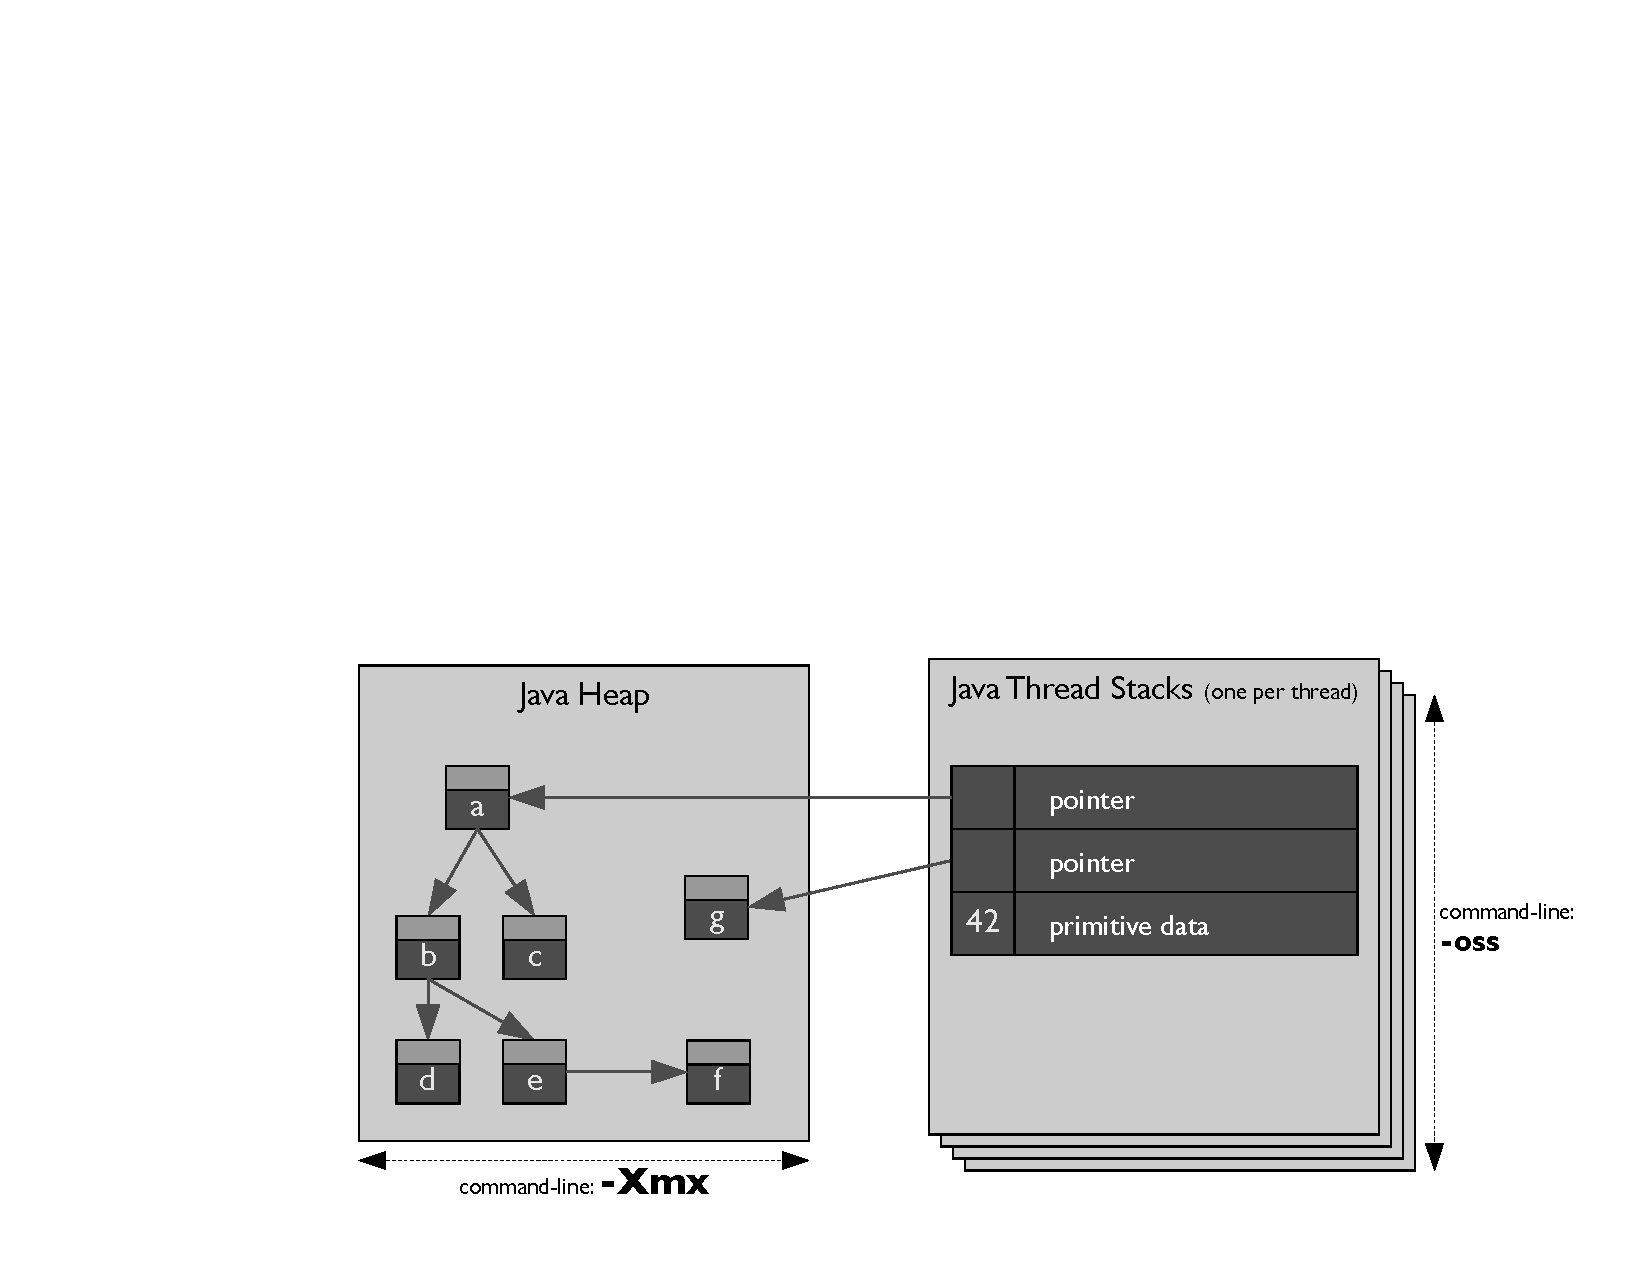
\includegraphics[width=0.575\textwidth]{part2/Figures/lifetime/heaps_and_stacks_java}}
	
\begin{subfloat}
\begin{minipage}[b]{0.4\textwidth}
\begin{shortlisting}
class B {
  D d; 
  E* e;
}
void foo() {
  A *a = new A();
  F f();
  G g();
  a->b->e->f = &f;
  ...
}
\end{shortlisting}
\end{minipage}
\caption{When coding in C++.}
\end{subfloat}
	\subfigure[When
	using
	native code, such as when coding in C,
	the stack can also contain allocated storage ({\tt
	structs}), and allocated storage can include
	other structures that have been inlined ({\tt d} has been inlined into {\tt
	b}); there are no headers in C, since it is not a managed language.
	]{\label{fig:heaps_and_stacks_C}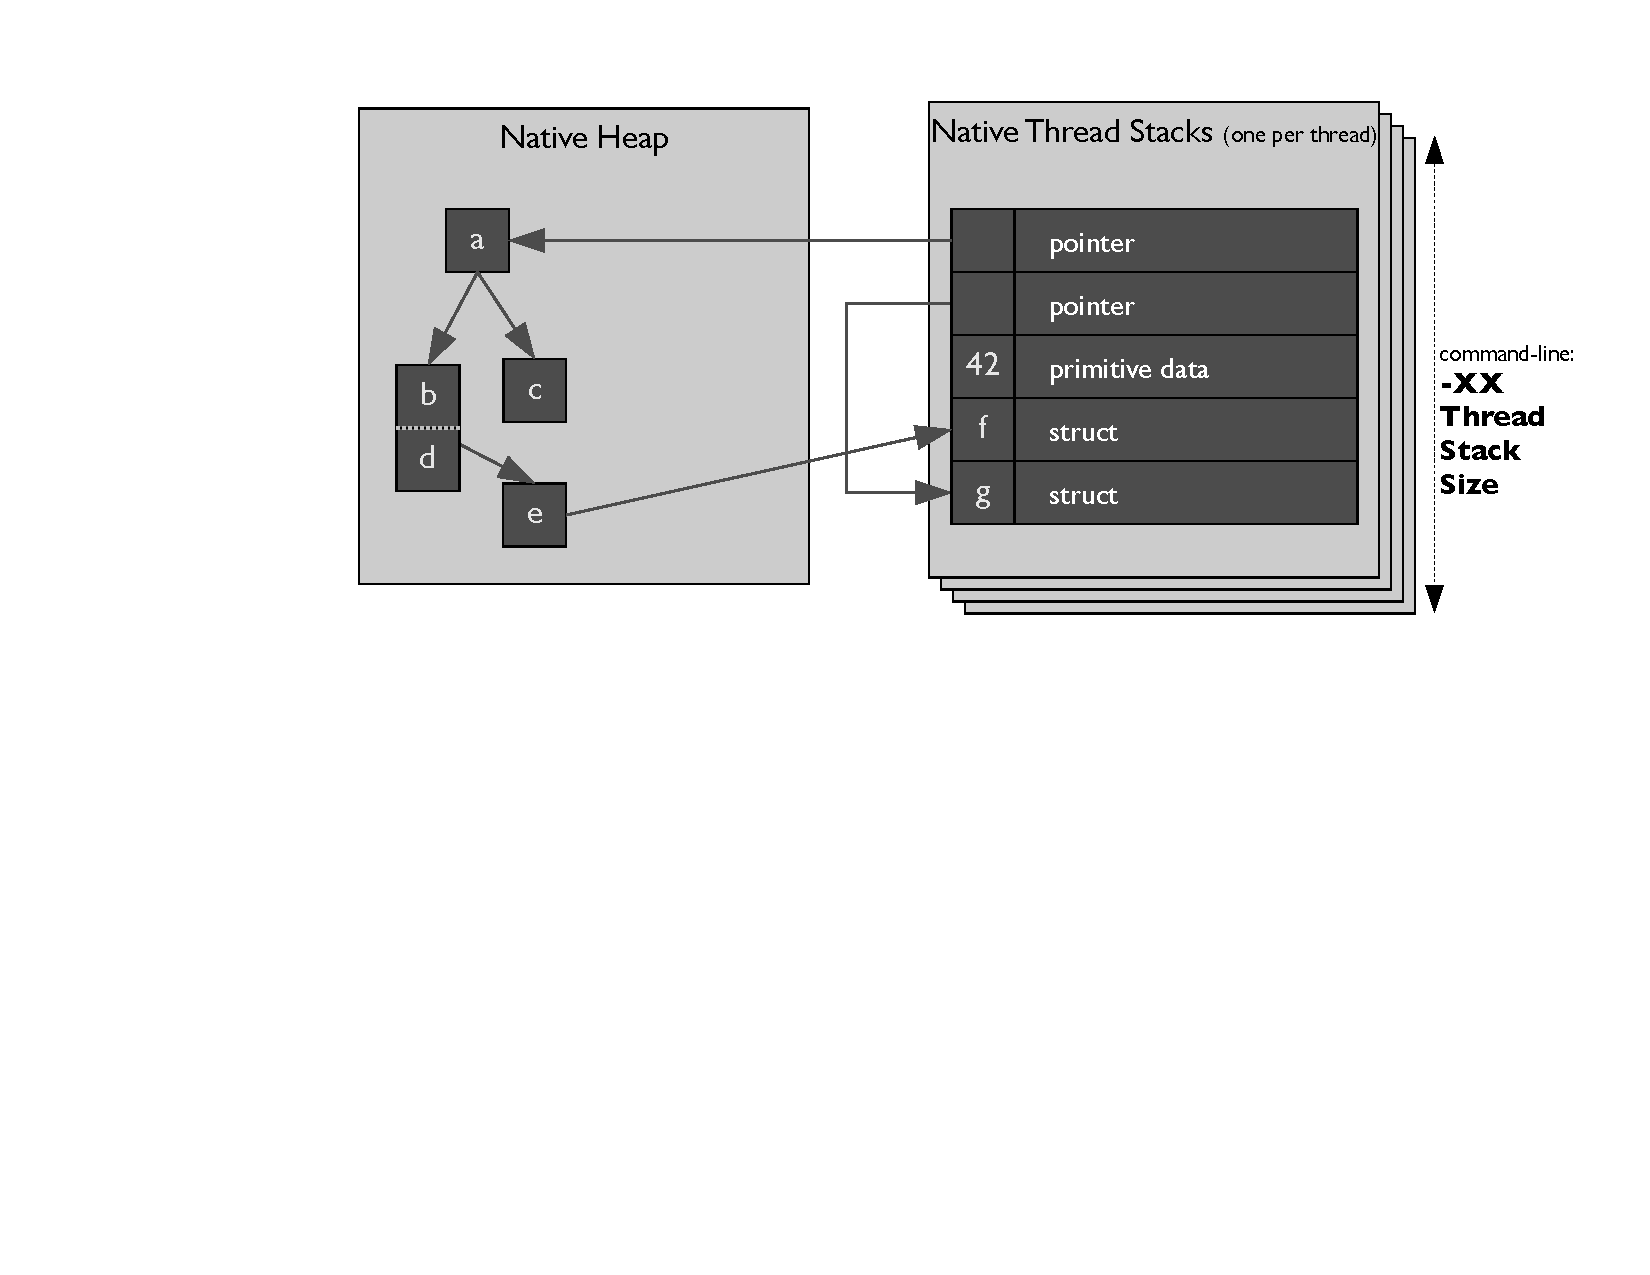
\includegraphics[width=0.575\textwidth]{part2/Figures/lifetime/heaps_and_stacks_C}}
	\caption{Heaps and Stacks, in Java versus in the C languge.}
\end{figure}



\begin{figure}
\centering
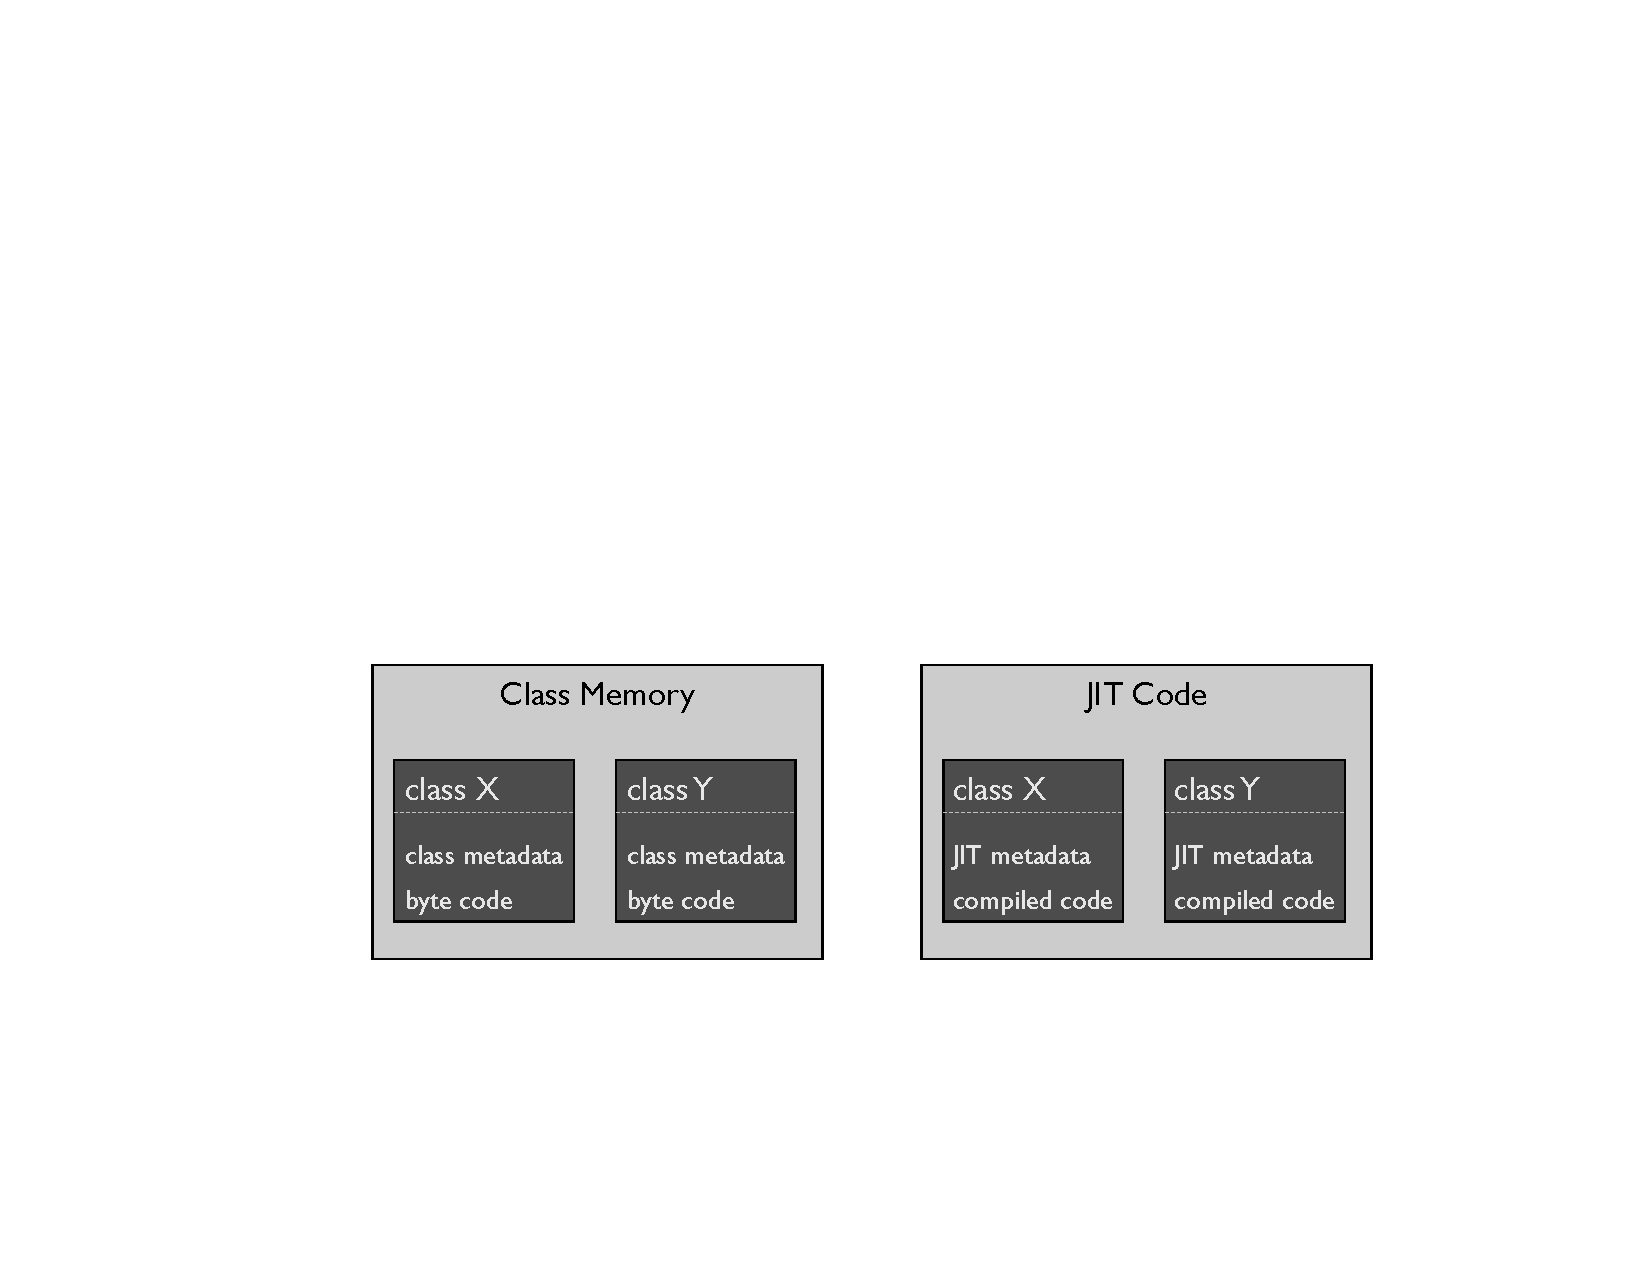
\includegraphics[width=0.75\textwidth]{part2/Figures/lifetime/heaps_and_stacks_classes}
\caption{The \jre also manages classes and compiled code, but in separate
	heaps. With some \jres, this data is combined into a single heap, called the
	\emph{Permspace}
	heap,
	which
	is
	sized
	via
	{\tt
	-XX:MaxPermSize}.}
\label{fig:heaps_and_stacks_C}
\end{figure}

\paragraph{The Java Heap vs. The Native Heap}



%Designing a lifetime management strategy requires that you take the tools that
%Java provides, and combine them with other strategies implemented on top of
%Java. The built-in mechanisms handle some aspects of the common patterns of
%object lifetime. 

%This chapter introduces the basics of the garbage collector, and how the Java
%managed runtime governs object lifetimes. Then, it walks you through the
%lifecycle of typical objects from allocation to eventual garbage collection. If
%you are comfortable with the basics of memory management, you may discover that
%you can skip to the next chapter.

\paragraph{The Garbage Collector}
The garbage collector is the mechanism for determining when an object should be
reclaimed. It is governed by a number of configuration choices that you can make.
These configuration choices guide the schedule that the collector follows. This
includes, for example, the frequency of collection and the lengths of pauses your
application experiences. In any case, the collector will obey some basic
principles, dictated by how your data structures are interconnected, when
determining \emph{what} to collect.

%\paragraph{What a Collection Collects: Reachability and Unique Ownership}
Each time a garbage collection occurs, the collector inspects the heap for
possibly \emph{live} objects. The collector treats the heap as a graph of
objects. The nodes are the objects themselves, and the edges are field or array
slots that result in a pointer from one object to another. \index{Heap, as a
graph of objects} Recursively, an object is live either if it is a referenced
either by a live object, or, in the base case, by a \emph{root}. The roots of
garbage collection are those that come from outside the Java space, and include:
objects serving as monitors, objects on the stack of a method invocation in
progress, and references from native code via the Java Native Interface (JNI).
Every other object not live, in this sense, are ready for collection; they are
garbage.

\begin{figure}
\centering
	\subfigure[A live data
	structure.]{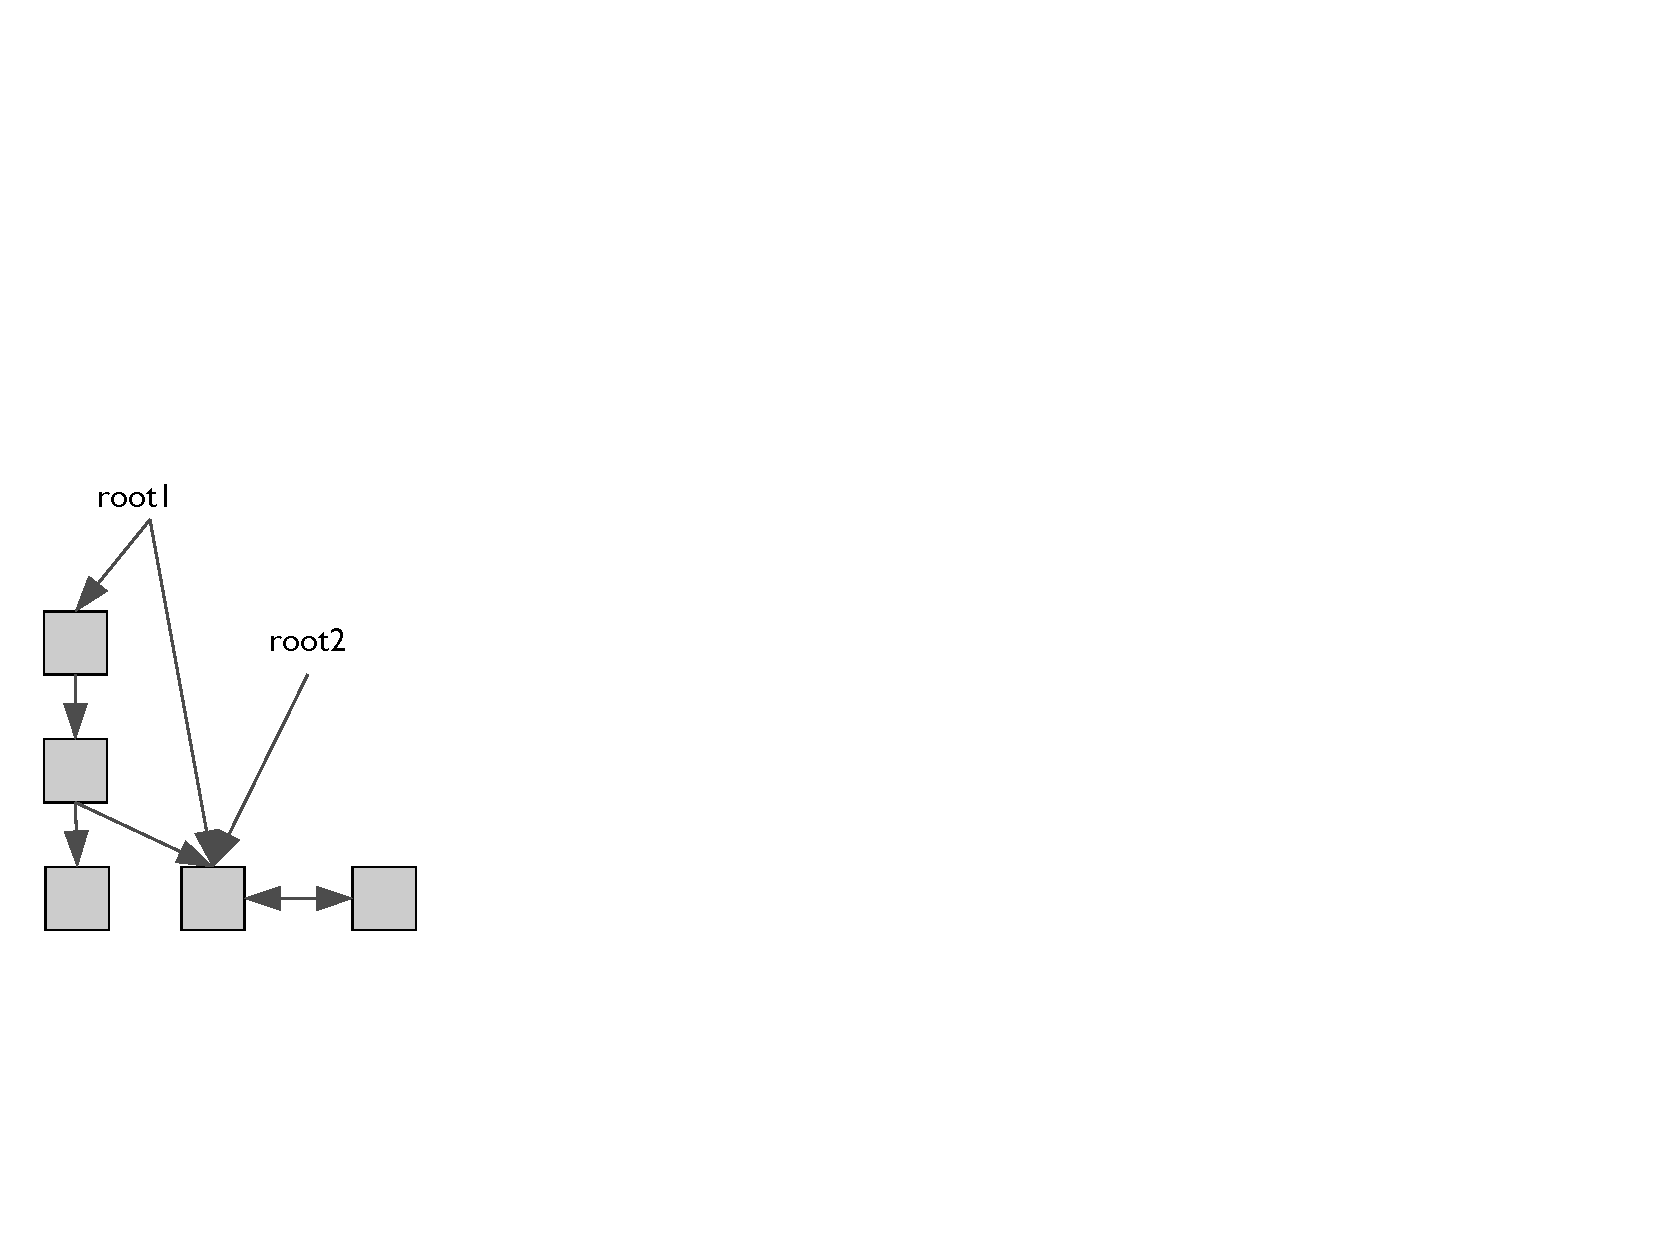
\includegraphics[width=0.3\textwidth]{part2/Figures/lifetime/reachability1}}
	\hspace{0.18\textwidth}
	\subfigure[Then, the dominating reference is
	clipped.]{\label{fig:reachability-b}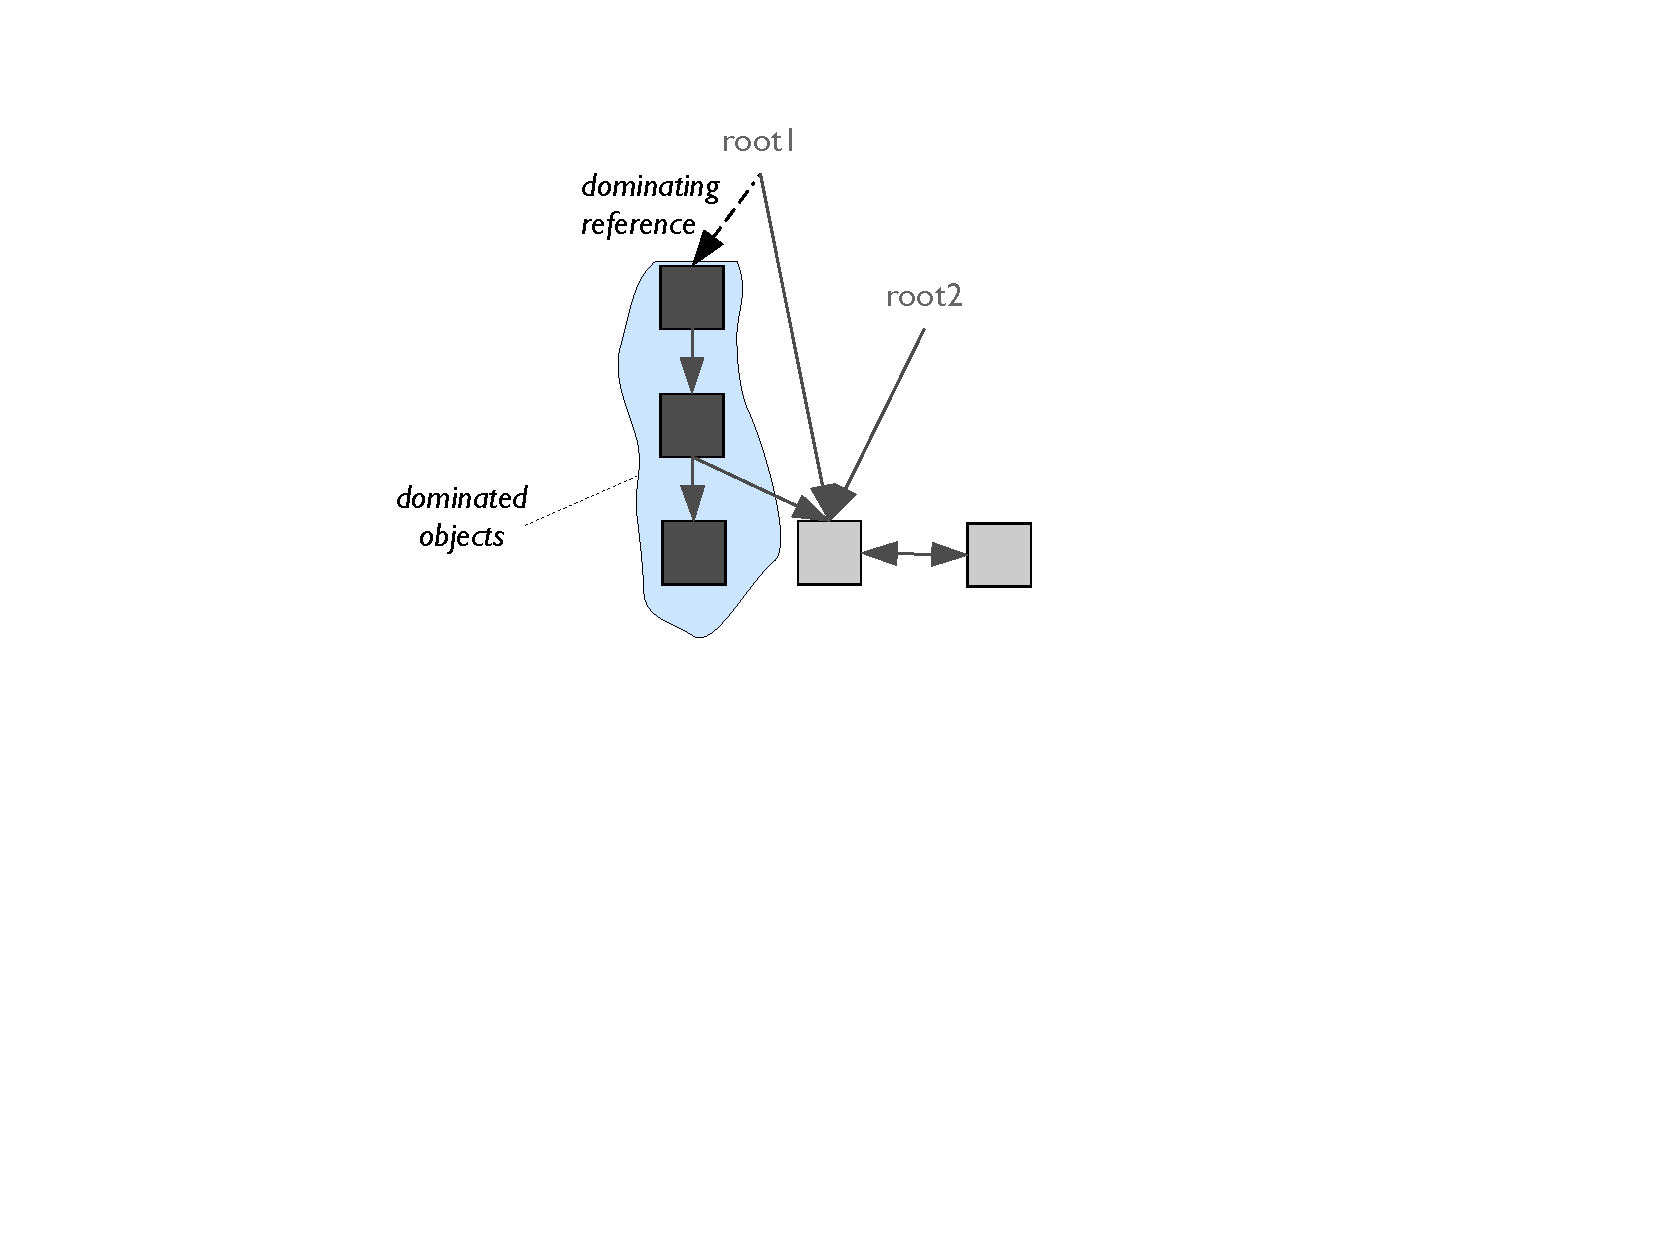
\includegraphics[width=0.445\textwidth]{part2/Figures/lifetime/reachability2}}
	\caption{The garbage collector uses the references between objects to
	determine what objects are collectable. The data structure on the left is
	filled entirely with live objects. The one on the right, after a link is
	clipped, now contains some collectable objects; all objects reachable only by
	traversing a \emph{dominating reference}, i.e. those \emph{dominated objects},
	will be collectable, as well.}
	\label{fig:reachability}
\end{figure}

This recursive aspect can also be expressed in terms of \emph{reachability}.
\index{Reachability} The live objects are those objects reachable, by following a
chain of references, from some root. \autoref{fig:reachability} illustrates a
simple data structure, and shows which part becomes collectable when a reference
is set to null, or ``clipped''. When the indicated reference is clipped, there is
no chain of references from a root to the shaded region of objects.

Reachability is the graph property that determines what objects are still live.
This is all the garbage collector cares about, finding the objects that need to
be kept around. It is also helpful for programmers to know which objects become
dead as the result of a pointer being clipped. The objects within the shaded
region of \autoref{fig:reachability-b} have the property that each is reachable
\emph{only} from the clipped reference. That clipped reference is the unique
owner of the shaded objects. The graph property that describes unique ownership
is called \emph{dominance}; \index{Dominance} the clipped reference is said to
dominate those objects that it uniquely owns.

\section{The Object Lifecycle}
\paragraph{How to Free an Object in Java}
\label{sec:natural-lifetime}
\index{Natural Lifetime of Objects}

If you wish an object's storage to be reclaimed, you must take some care. To do
so in a language like C is simple, if bug prone. When you call \code{free} on any
pointer to a dynamically allocated memory region, memory is immediately available
for subsequent use.\footnote{It is possible to run a C program with a
special \code{malloc} library that introduces a simplified form of garbage
collection.} A C style of memory management comes with well known risks, and
commonly leads to memory errors. For example, memory might be deallocated more
than once, or variables that do not point to the start of an allocated region
might be passed to \code{free}. Still, using \code{free} is straightforward to
use, and immediate in effect.

In Java, you are immune from these problems, but there is no way to return memory
for immediately use in future allocations. Instead, you indicate, either
implicitly or explicitly, that objects are no longer needed. The explicit
mechanism is to set references to null. To do so implicitly, there are several
devices at your disposal. This section describes the details of both.

It is important to remember that in contrast to C, all means of indicating an
object is no longer needed have a certain degree of delay. There are delays of
two sorts. First, if you rely on the implicit mechanisms for indicating an object is no
longer needing, there is often a delay from its last use to this point. Second,
there is a delay from the point at which you indicate an object is no longer
needed until its storage is reclaimed.

\paragraph{The Lifecycle of an Object}
These two delays are but a part of the larger lifecycle that every Java object
goes through, from creation to reclamation. In a well-behaved application, an
object's lifetime spans its allocation, use, and the short period during which
the \jre takes control and reclaims the space. For some subset of an object's
actual lifetime, that is the time from creation to reclamation, your application
will make use of the data stored in its fields. \autoref{fig:typical-lifecycle}
illustrates the lifecycle of a typical object in a well behaved application.

\begin{figure}
	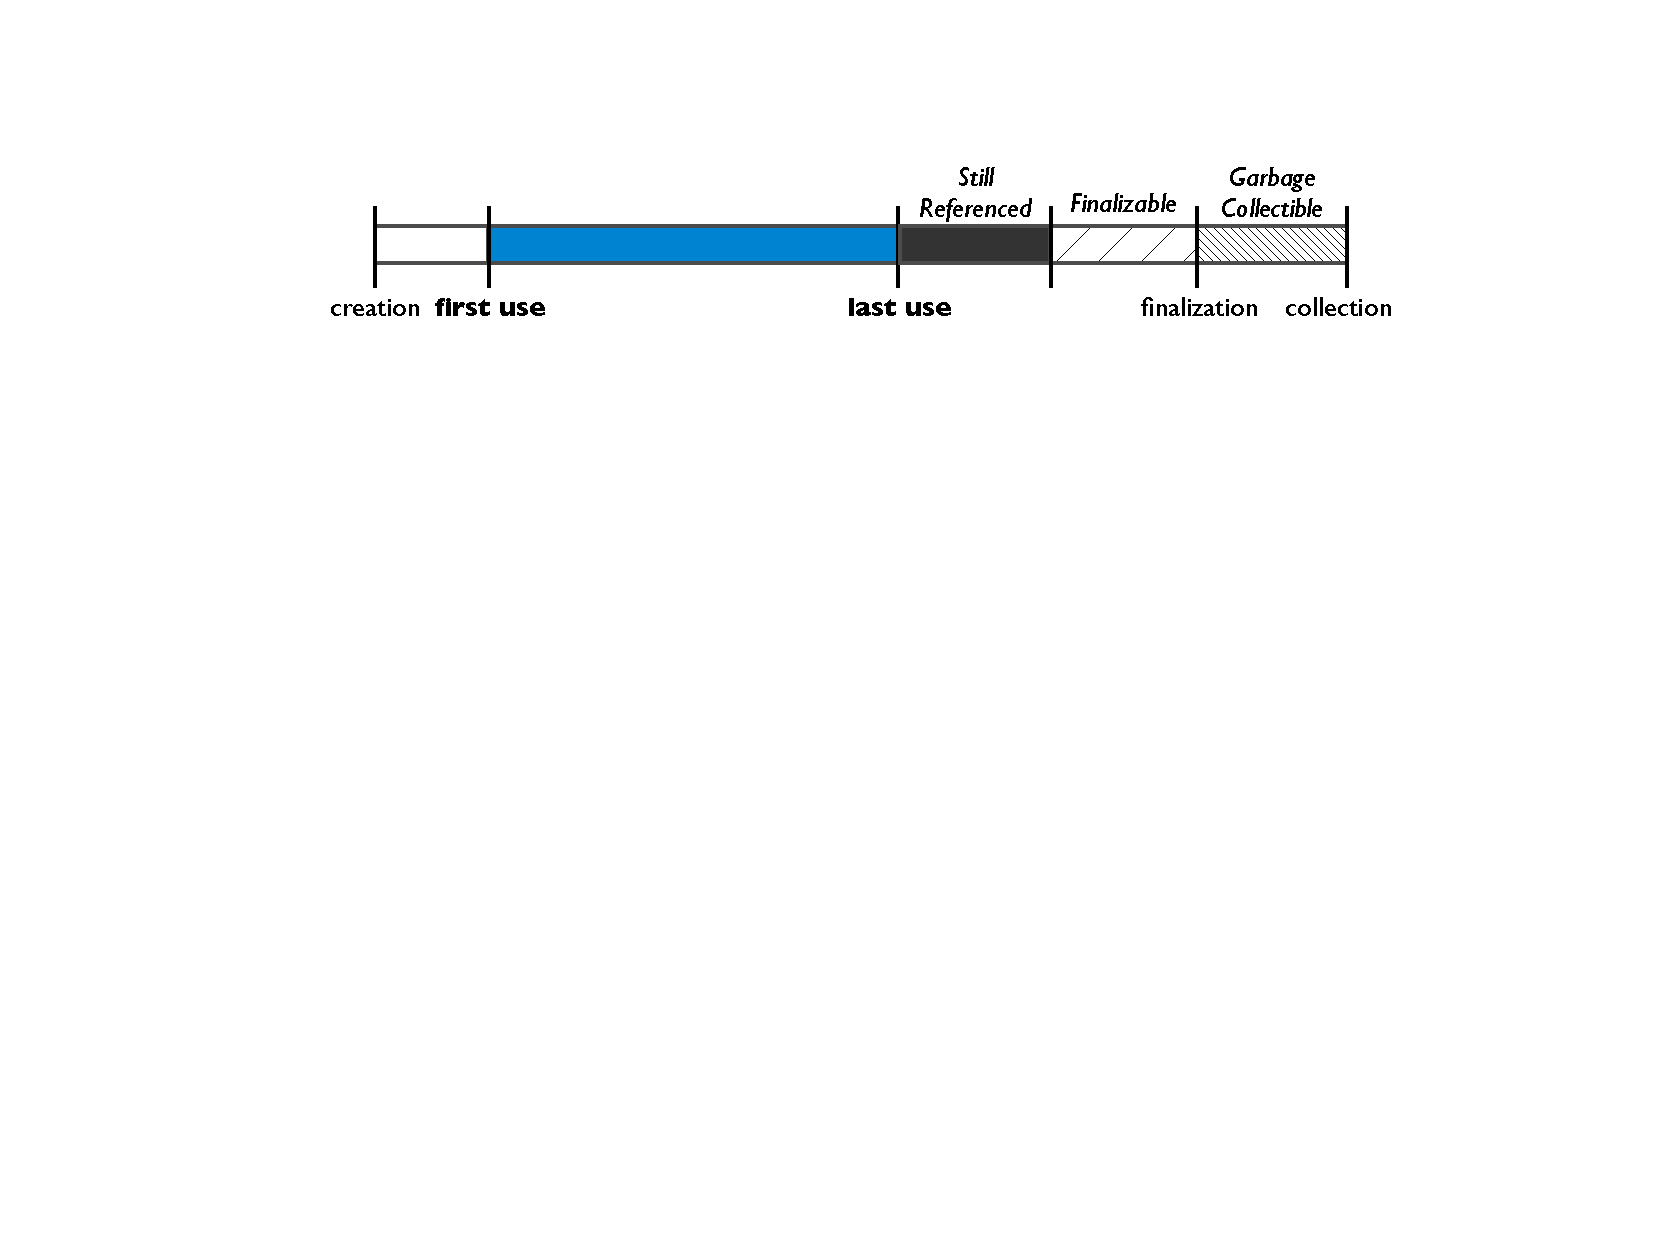
\includegraphics[width=0.9\textwidth]{part2/Figures/lifetime/object-lifecycle}
	\caption{Timeline of the life of a typical object.}
	\label{fig:typical-lifecycle}
\end{figure}


\begin{example}{Parsing a Date} Consider a loop that shows an easy way to parse
a list of dates. What objects are created, and what are their lifetimes?
\begin{shortlisting}
for (String string : inputList) {
	ParsePosition pos = new ParsePosition(0);
	SimpleDateFormat parser = new SimpleDateFormat();
	System.out.println(parser.parse(string, pos));
}
\end{shortlisting}
\end{example}

For each iteration of this loop, this code takes a date that is represented as a
string and produces a standard Java \class{Date} object. In doing so, a number of
objects are created. Two of these are easy to see, in the two \code{new} calls
that create the parse position and date parser objects. The programmer who wrote
this created two objects, but many more are created by the standard libraries to
finish the task. These include a calendar object, number of arrays, and the
\class{Date} itself. None of these objects are used beyond the iteration of the
loop in which they were created. Within one iteration, they are created, almost
immediately used, and then enter a state of drag.

\callout{drag}{Memory Drag}{
\index{Drag}
At some point, an object will never be used again, but the \jre doesn't yet know
that this is the case. The object hangs around, taking up space in the Java heap
until the point when some action is taken, either by the \jre or by the
application itself, to make the object a candidate for reclamation. The interval
of time between its last use and ultimate reclamation is refered to as
\emph{drag}.}

The \code{pos} object represents to the parser the position within the input
string to begin parsing. The implementation of the \code{parse} method uses it
early on in the process of parsing. Despite being unused for the remainder of the
parsing, the \jre does not know this until the current iteration of the loop has
finished. For this duration of time the object is in a kind of limbo, where it is
referenced but never be used again. This limbo time also includes the entirety of
the call to \code{System.out.println}, an operation entirely unrelated to the
creation or use of the parse position object. Once the current loop iteration
finishes, these two objects will become candidates for garbage collection.

\begin{figure}
	\centering
	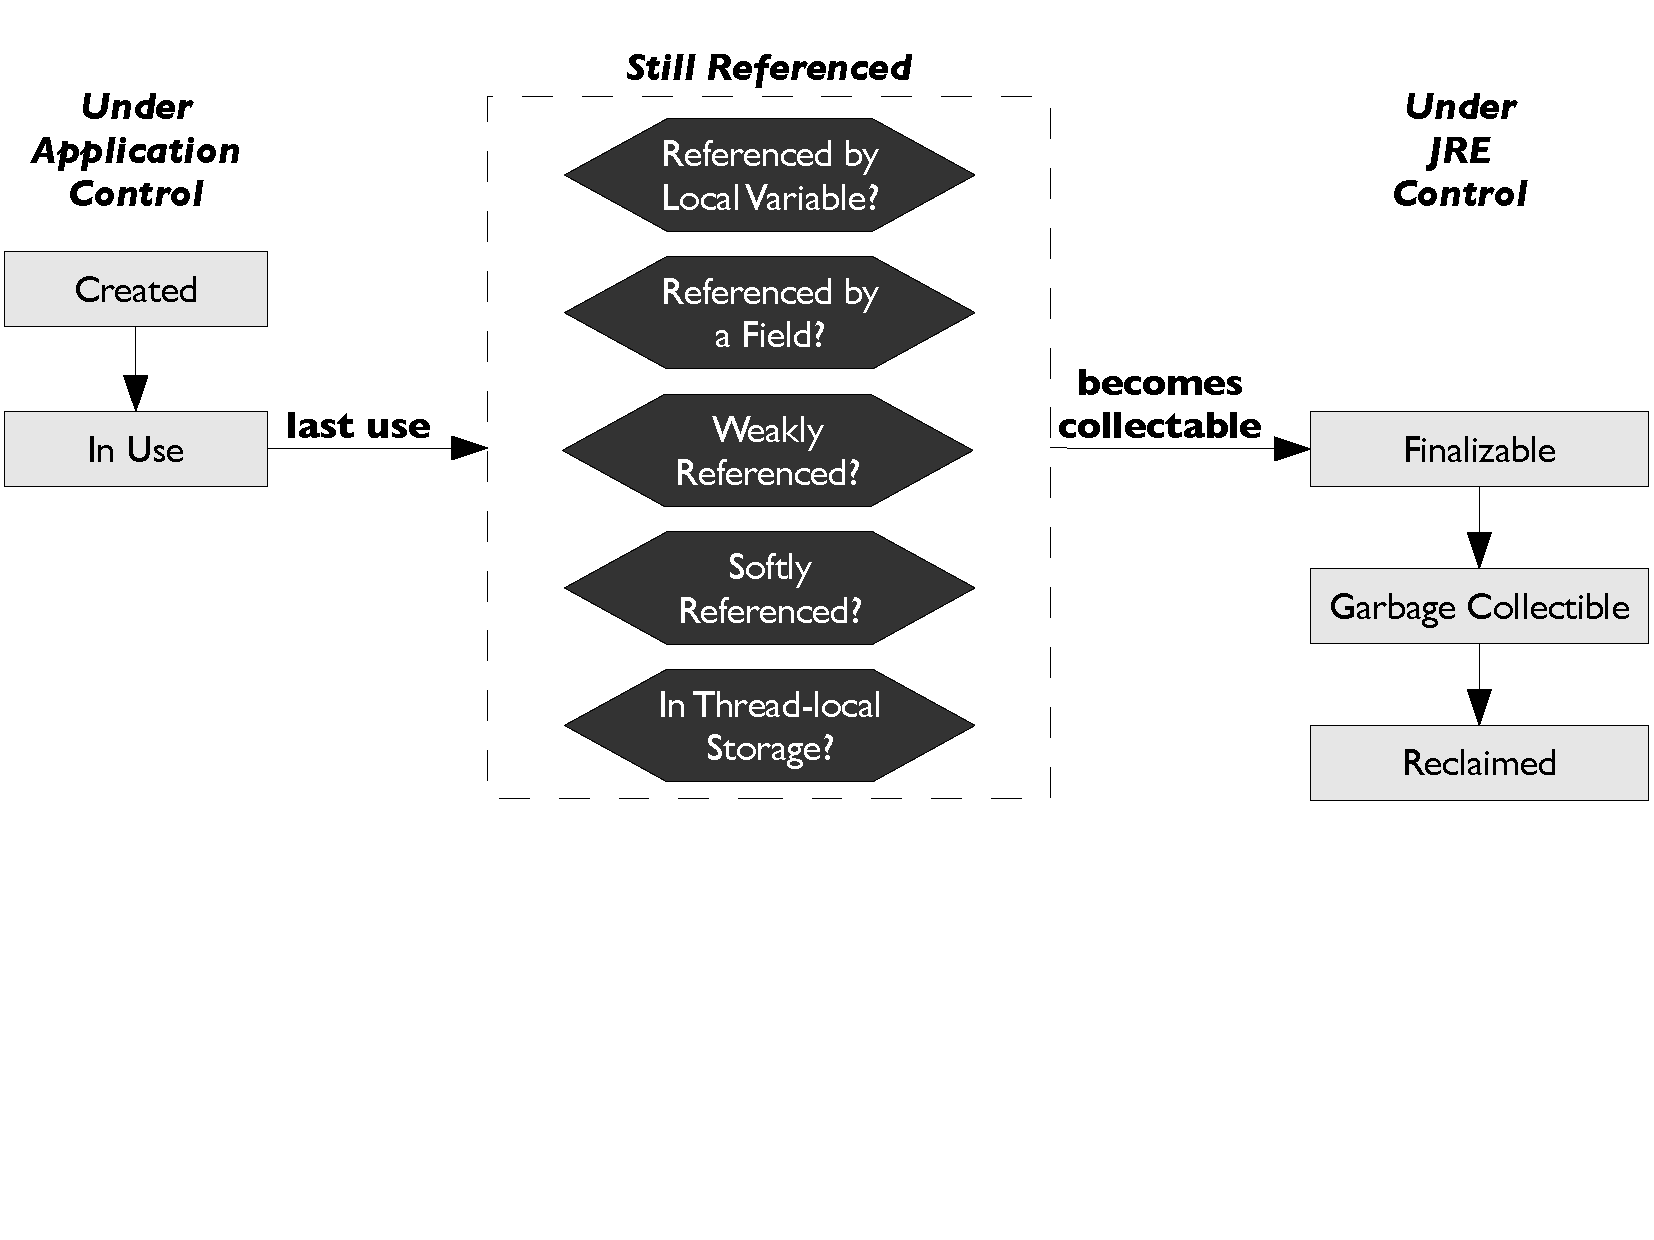
\includegraphics[width=\textwidth]{part2/Figures/lifetime/states}
	\caption{After its last use, an object enters a kind of limbo: the application
	is done with it, but it is not yet a candidate for garbage collection. When an
	object exits this limbo depends on the way it is referenced by your
	application.}
		\label{fig:limbo-exit}
\end{figure}

Depending on how the object is referenced by your application, it will
transition from in-use to garbage-collectable in a different manner. There are
eight ways an object may be referenced. It can be referenced by a:

\begin{enumerate}
  \item local variable of a method
  \item static field of a class
  \item instance field of a \class{java.util.ref.WeakReference} object
  \item instance field of a \class{java.util.ref.SoftReference} object
  \item instance field of a \class{java.util.ref.PhantomReference} object
  \item \tls
  \item instance field of any other object
  \item some combination of the above
\end{enumerate}

The first seven are cases of unique ownership of an object. There exists
only one path, via that particular reference, to reach the object. The eight case
is one of \emph{shared} ownership. After your program creates an object, it
references the object in one or more of these eight ways. The ownership of an
object may vary over time --- as your program runs, these references will come
and go. After some time, program execution may reach a point where the object is
no longer under application control. At this point, the \jre is now in charge of
its lifetime. For example, if the only reference to an object is from a field of
some other object, and your code reassigns that reference to \code{null}, this
becomes a point of transition, from application control to \jre control. Each of
the eight ways of referencing an object comes with its own guidelines as to when
this transition occurs. \autoref{fig:limbo-exit} and \autoref{tab:limbo-exit}
summarize how an object transitions to \jre control. The following code gives
examples of these eight patterns of ownership:
\lstset{numbers=left,numbersep=12pt,numberstyle=\tiny\textsf}
\begin{shortlisting}
class Foo {
   void bar(Object argument) {
      Object localVariableReference1 = new ...;
      threadLocal1.set(argument);
      threadLocal2.set(new ...);
      localVariableReference1 = null;
      for (...) {
         Object localVariableReference2 = new ...;
         ...
      }
   }

   static Object staticField = new ...;
   Object instanceField = new ...;
   Reference weak = new WeakReference(instanceField);
   Reference soft = new SoftReference(instanceField);
   Reference phantom = new PhantomReference(instanceField);
   ThreadLocal threadLocal1 = new ThreadLocal();
   ThreadLocal threadLocal2 = new ThreadLocal();
}
\end{shortlisting}
\lstset{numbers=none}
% Still, one can't always rely on automatic mechanisms to guide an object out of
% limbo in a timely fashion.

\begin{table}
\centering
	\begin{tabular}{ll} \toprule uniquely owned by  & 
	when object becomes candidate for reclamation \\ \cmidrule(r){1-1}
	\cmidrule(l){2-2}
			%
			nothing & immediately
        	\\
        	%
        	local variable & after scope exits, e.g. method returns
        	\\ \addlinespace
        	%
        	instance field of an object & 
        	when that object becomes reclamation candidate
        	\\
        	%
        	static field of a class &
        	when that class is unloaded
        	%
        	\\ \addlinespace
        	field of \class{WeakReference} & immediately
        	%
        	\\
	       	\ldots with \class{ReferenceQueue} &
        	immediately placed on queue, then after queue is polled
        	%
        	\\ \addlinespace
        	field of \class{SoftReference} & approximately
        	LRU%$^{**}$
        	%
        	\\
	       	\ldots with \class{ReferenceQueue} &
        	after LRU, placed on queue, then after queue is polled
        	%
        	\\ \addlinespace
        	entry in \tls & when that thread dies
        	%
        	\\ 
        \bottomrule
    \end{tabular}
	\caption{When an object becomes a candidate for reclamation. The dominating 
	reference can be explicitly overwritten, e.g. by your code expliclty assigning the
	reference to \code{null}. Otherwise, an object only automatically becomes a
	candidate under the restricted circumstances shown here.
%	The point when an object exits limbo depends on 
	%decisions under programmer control: it depends on how the object is
	%referenced.
	%older {\jre}s	use very poor heuristics for handling soft references; see the
	% body for more detail.
	%, it will be reclaimed
	%under certain rules, or may be part of a memory leak
	}
	\label{tab:limbo-exit}
\end{table}

\paragraph{The Lifetime of Local Variables}
\label{sec:lifetime-of-locals}
Variables that are declared within a method body often have a lifetime that is
bound to, at most, the duration of an invocation of that method.
% If an object is uniquely owned by a local variable of a method, the \jre will
% begin to consider reclaming its storage no sooner than when the local
% variable's scope exits.
Common examples of this are local variables, loop variables, and variables
declared within some inner scope such as within the body of a loop or \code{if}
statement. For these variables, when a loop continues to the next iteration as in
the case of \code{localVariableReference2}, when the body of a clause of an
if/then/else statement finishes, or when the method invocation returns as in the
case of \code{localVariableReference1}, there is a good chance that the object
referenced by that variable will be reclaimable.

There are situations where an object may \emph{escape} the local scope in which
it was declared.\index{Escaping Objects} In these cases, the object has
\emph{shared ownership}\index{Shared Ownership} until this local scope exits.
See below for further discussion of shared ownership. This is an example of an
object escaping a local variable scope, so that it is, for the duration of that
local scope, also owned by a static field of a class object:
\begin{shortlisting}
class Foo {
   static Object static_obj;
   
   void foo() {
      Object obj = new Object();
      static_obj = obj;
      ... // uses of obj
   } // obj scope exits, but static_obj ownership persists
}
\end{shortlisting}
The next section discusses the lifetime of static fields.

The minimum that the Java language specification requires is that non-escaping
objects that are declared within some scope inside of a method will be
reclaimable by the time that scope exits. Many modern \jres try to optimize by
inferring, when they can, the line of code at which an object will certainly
never be used again. For this reason, some (but not all!) sources of memory
drag\index{Drag} that would have been a problem with older \jres, are no longer
an issue. For example, you can run this test program and, by inspecting the
output, determine whether your \jre is performing this kind of optimization:
\begin{shortlisting}
/* Test for whether the optimizer detects that obj is reclaimable before the end of this method */
static public void main(String[] args) {
   Object obj = new Object() {
      protected void finalize() {
         System.out.println("Finalized");
      }
   };
   System.out.println("StartOfLoop");
   for (int i = 0; i < 1000000; i++) {
       new HashSet().add(i);
   }
   System.out.println("EndOfLoop");
}
\end{shortlisting}
If you see the \code{Finalized} message before the end of loop message, this is a
sure sign that the \jre is being clever. Be careful to remember that seeing the
finalized message is definitive evidence, but not seeing that message might only
mean that your loop doesn't iterate enough times to cause a garbage collection to
occur. You may need to experiment with the number of loop iterations, before
coming to a conclusion.

\paragraph{The Lifetime of Statics, and Class Unloading}
\index{Class Unloading}
\index{Static fields}

The \jre allocates memory for every class, to store its static fields, such as
the one on line 13 in the above example. This memory, to store all static fields
plus some bookkeeping information, is often referred to as the \emph{class
object} for the class.\index{Class Objects} It is possible for the same class to
be loaded into multiple class loaders; in this way, using more than one class
loader lets you avoid the problem of colliding use of static fields in separately
developed parts of the code. A static field therefore only exits scope when the
class object is reclaimed, which occurs when the respective class is unloaded, by
the \jre, from its class loader. 

If a class is never unloaded, which is likely to the be case for your
application, then that class object will remain permanently resident. The
\emph{default} class loader, which is the one that will be used unless you
specify otherwise, never unloads application classes. 

If you need classes to be unloaded, then you must manually specify a class loader
to use. Unloading a class is then accomplished by ensuring that all references to
both the class object and your custom class loader, are set to \code{null}. This
will render the class unloadable, and will also render objects referenced by
static fields all classes loaded into that class loader as garbage collectable.
There exist module management systems, such as OSGi~\cite{OSGi_2007}, that
facilitate this task.

Due to these complexities, your design should generally anticipate that the
memory for these static fields is permanently resident. This means that any
static fields referencing an instance, rather than containing primitive data,
will render that instance also permanently resident. Unless, that is, you take
action to explicitly clip the static field reference, by assigning the field to
null. Otherwise, that instance will be forever reachable along a path from some
garbage collection root through the static field reference. In this way, storing
a reference in a \code{static} field of an class is one way to implement a
permanently resident lifetime policy.

\paragraph{The Lifetime of Instance Field References}

As long as an object \code{B} is dominated by an instance field of another object
\code{A}, then these two objects will live and die together. The only device at
your disposal to make \code{B} garbage collectable before \code{A} is to break
all paths of references from \code{A} to \code{B}. In simple cases, where
\code{B} is directly referenced by a field of \code{A}, then reassigning that
reference to \code{null} will do the trick. After doing so, the \code{B} object
will now be a candiate for garbage collection. 



%Every object created by your application lives for an interval of time from its
%creation to the point that the Java runtime gets around to collecting it. An object's {\em natural} lifetime is defined by the
%interval of time between its first and last necessary use. %cite drag paper
%here?








\begin{comment}
\begin{figure}
	\centering
%	\subfigure[The lifecycle of a typical object and its data.]{
	%\label{fig:typical-lifecycle1}
			%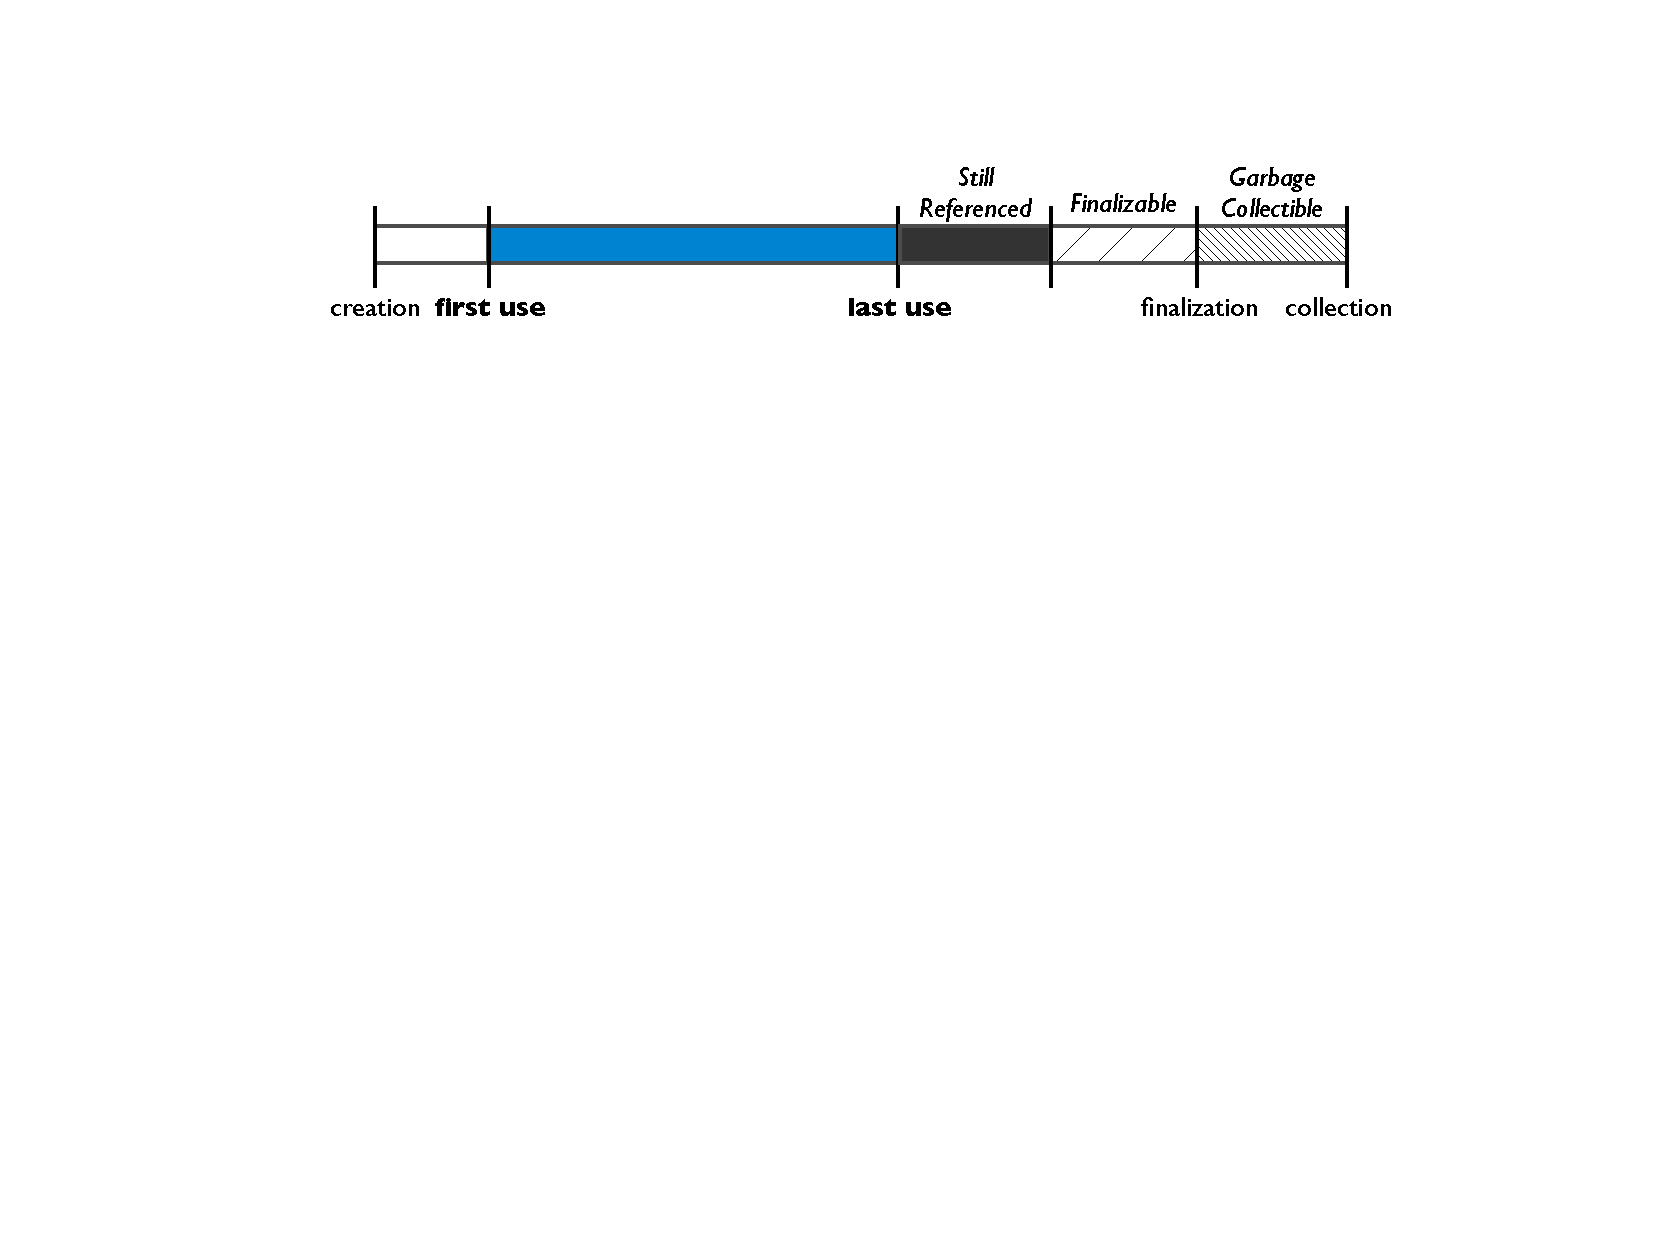
\includegraphics[width=0.95\textwidth]{part2/Figures/lifetime/object-lifecycle}
	%}
	\subfigure[A situation where there are long periods between uses of an
	object's data.]{
	\label{fig:typical-lifecycle2a}
		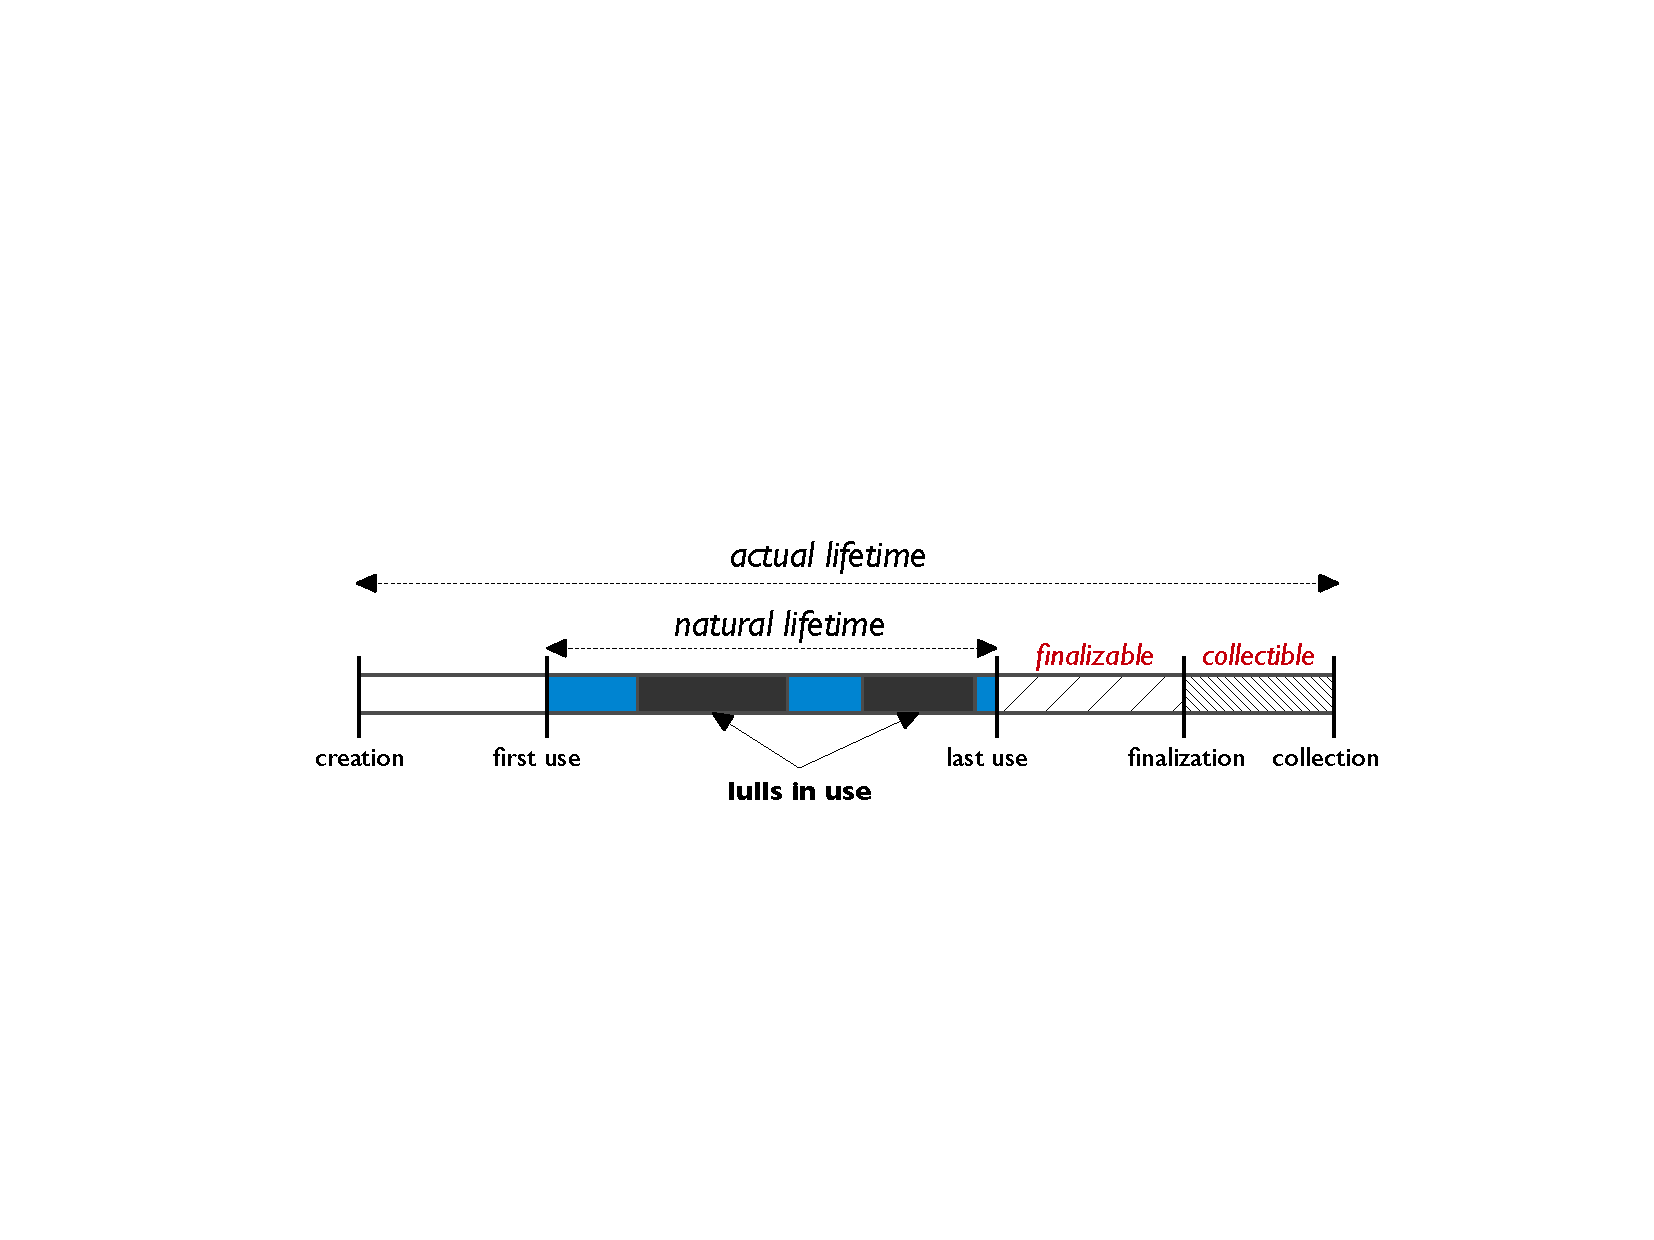
\includegraphics[width=0.95\textwidth]{part2/Figures/lifetime/object-lifecycle-lulls}
	}
	\subfigure[The lifecycle of the data  that is loaded from
	disk three times, and the objects that store it.]{
	\label{fig:typical-lifecycle2b}
		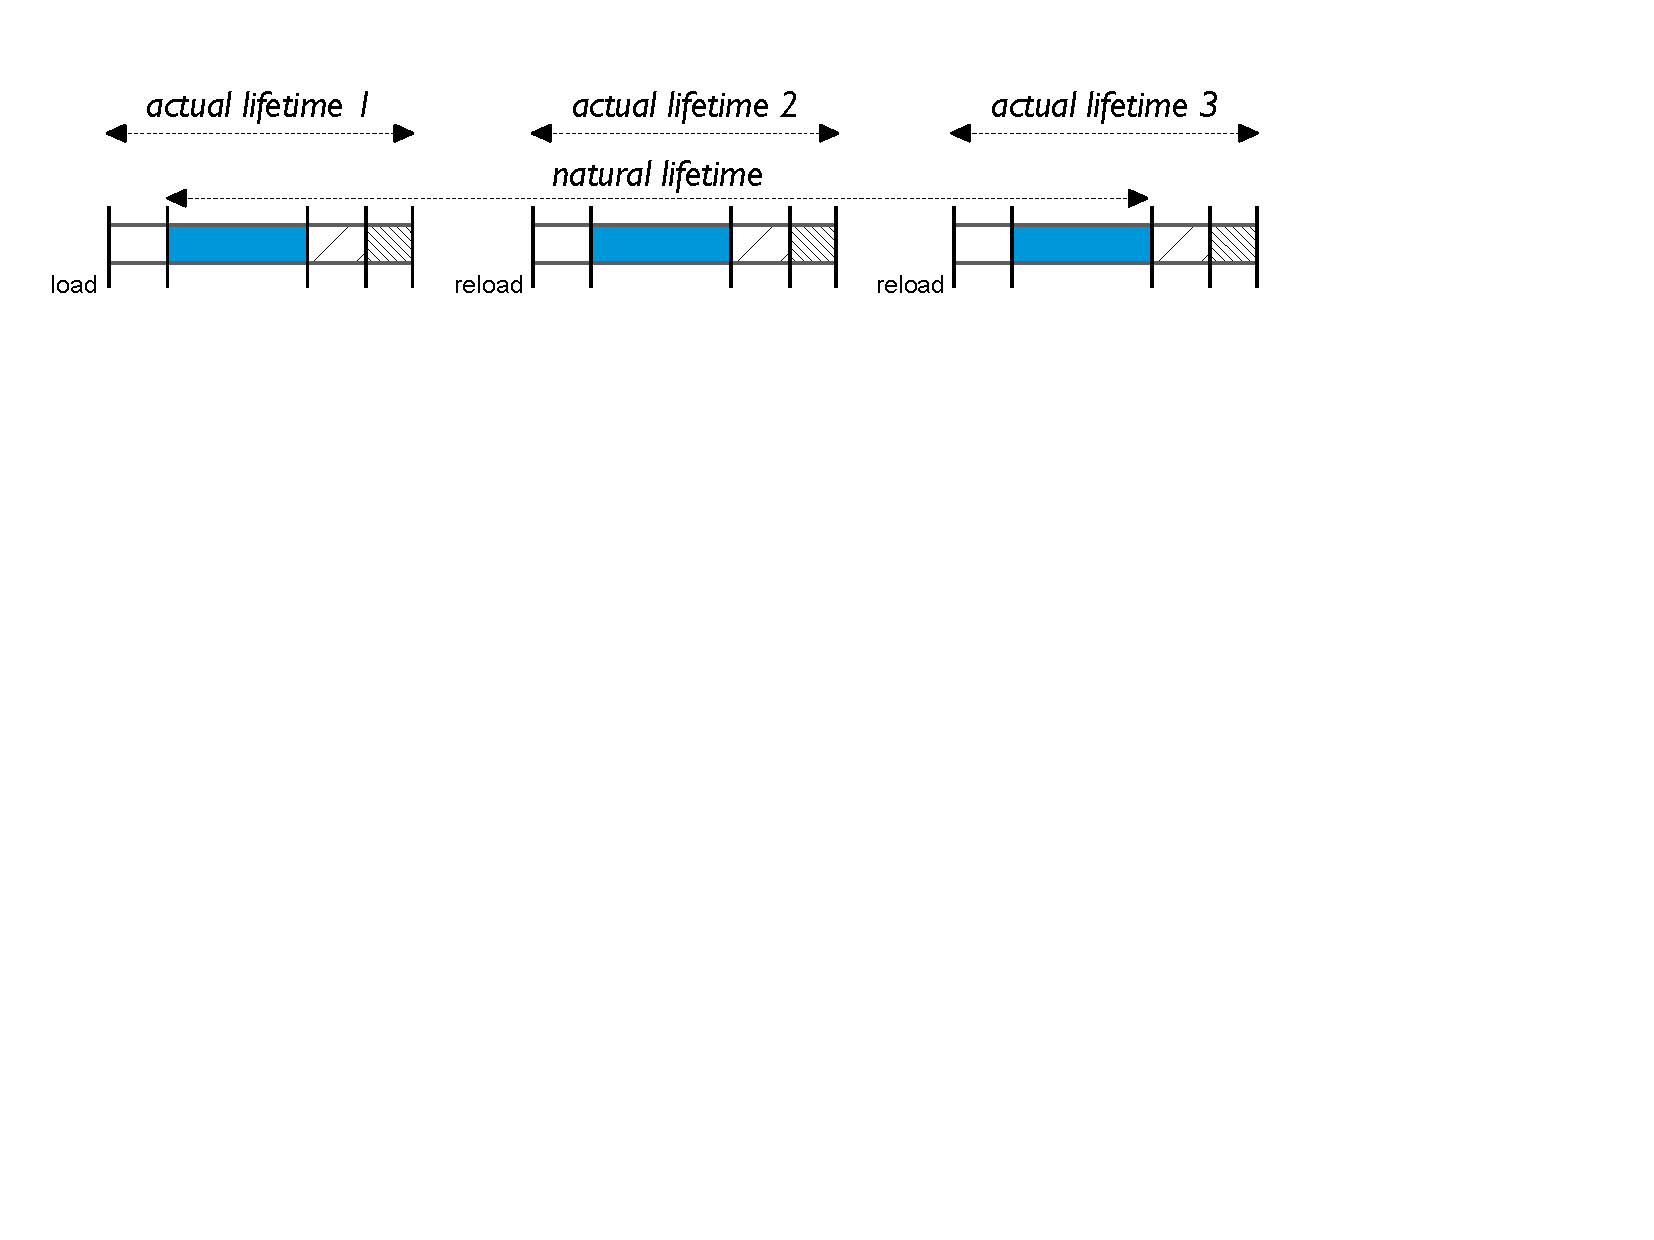
\includegraphics[width=0.9\textwidth]{part2/Figures/lifetime/object-lifecycle2}
	}
	\caption{Examples of Natural and Actual lifetimes.}
	\label{fig:typical-lifecycle2}
\end{figure}
\end{comment}


\paragraph{Shared Ownership}
\label{sec:shared-ownership}
\index{Shared Ownership}

When you invoke a library method, there is no way in Java to know what the called
method does with your object. It could very well squirrel away a reference to any
object reachable from arguments you pass to the invocation. Despite your best
efforts at keeping track of which references exist to an object, it can easily
become an uncontrolled mess once you pass these objects to third-party libraries.
In the above example, if you call the \code{parse} method of a
\class{SimpleDateFormat} object, the method contract says nothing about how it
treats the given string or \class{ParsePosition} passed as parameters. 
Consider the case where you need the string to become garbage collectable soon
after having parsed it, but the formatter maintains a reference in order to avoid
reparsing the same string in back to back calls. This calls
to mind the worst of the days of explicitly managing memory in a language like C.

In the case where there is more than one reference to the object, the story gets
more complicated. In contrast to C, where a \code{free} of \emph{any} pointer
suffices for deallocation, in Java \emph{all} references to an object must be
assigned to \code{null}. This is tricky in many cases, because it may not be easy
to know where all those references emanate from.
\autoref{fig:reachability-sharing} illustrates a situation where three references
must be clipped before an object, the darkly shaded one, becomes a candidate for
garbage collection. There are two other important things to note in this example.
First, just as in \autoref{fig:reachability-b}, after clipping the three
indicated references, an entire data structure, not just that darkly shaded
object, becomes a candidate for reclamation. This structure consists of the two
objects contained within the lightly shaded region. The second important thing to
note is that you needn't clip the backwards edge, or any edge contained entirely
within the data structure you no longer need.

\begin{figure}
\centering
\subfigure[Diamond sharing.]{
	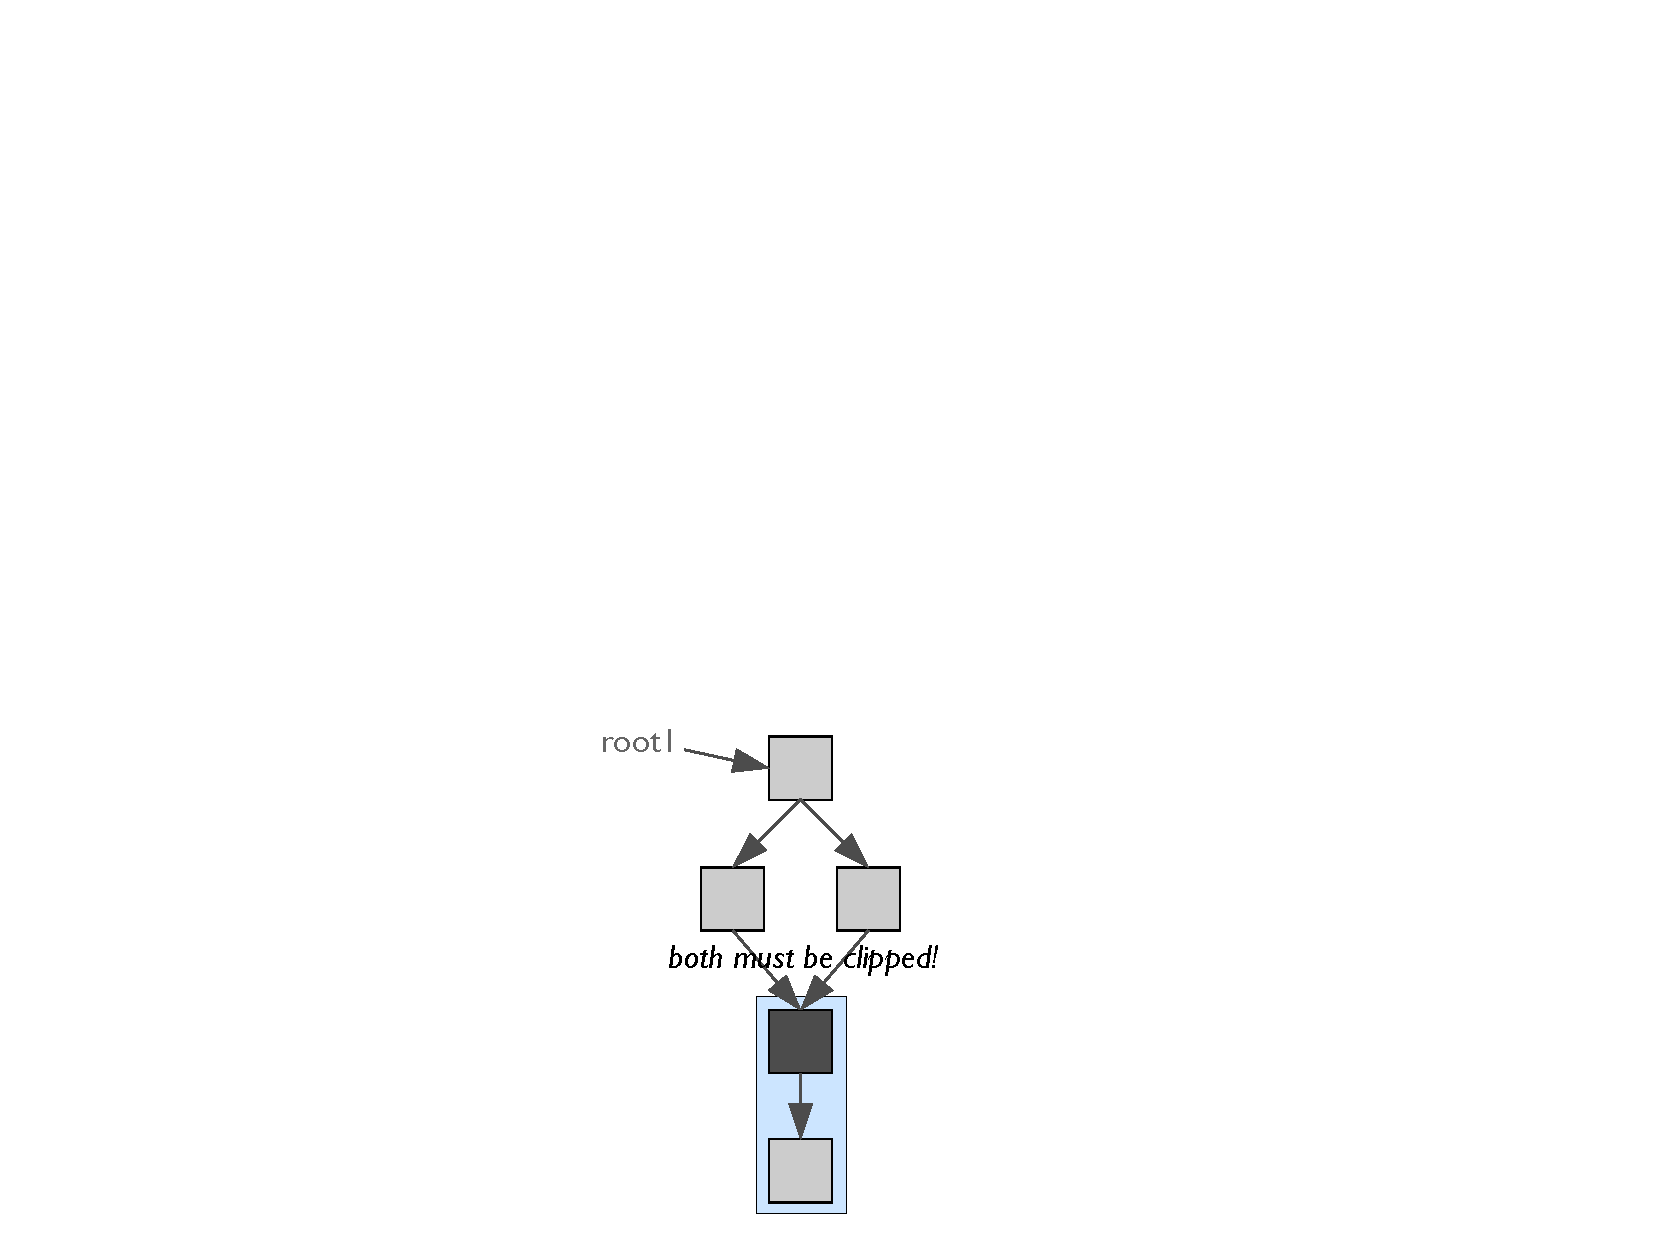
\includegraphics[height=0.25\textheight]{part2/Figures/lifetime/reachability4}
	}
\qquad
\subfigure[Root sharing.]{
	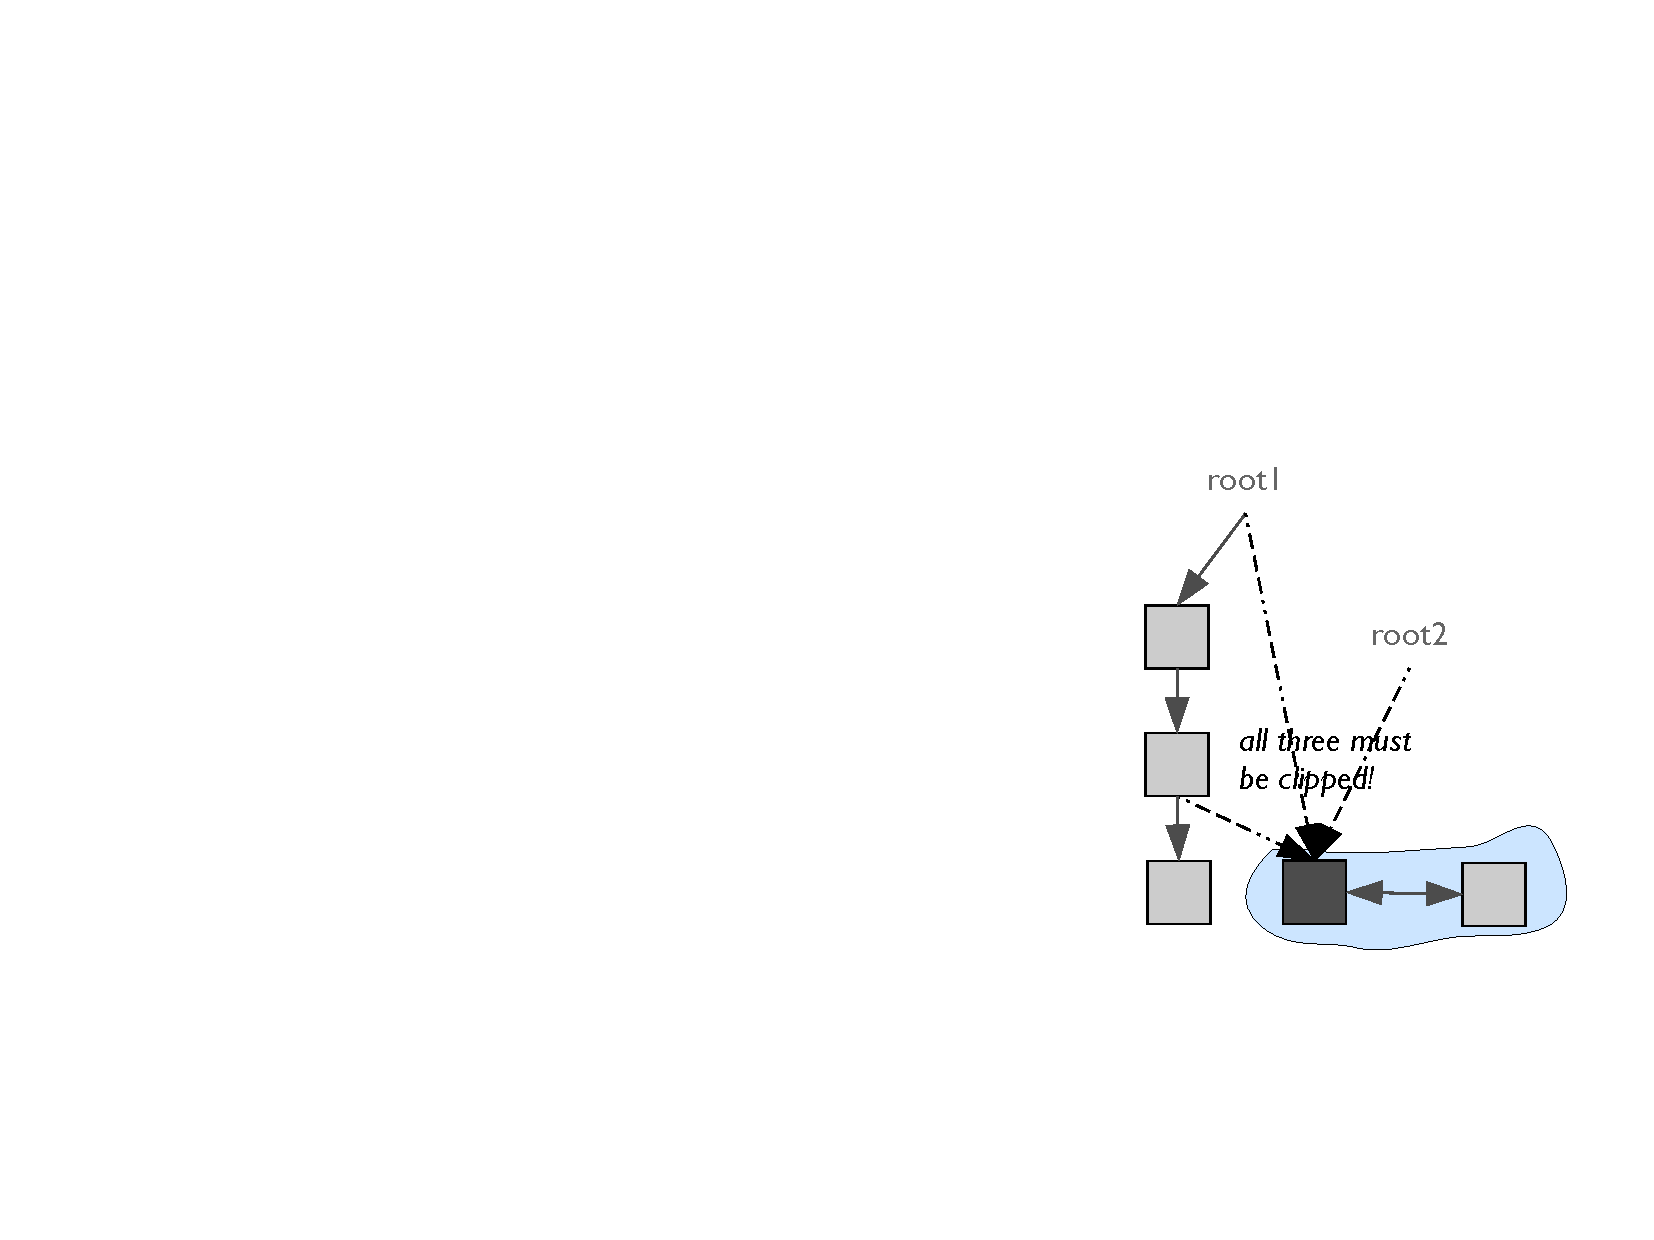
\includegraphics[height=0.22\textheight]{part2/Figures/lifetime/reachability3}
	}
	\caption{When an object is shared, such as the shaded ones shown
	here, care must be taken to clip all edges from emanating from outside of the
	region you wish to reclaim.}
	\label{fig:reachability-sharing}
\end{figure}

\section{Advanced Lifetime Management Features}
 
There are several important lifetime management policies that cannot be expressed
using normal mechanisms of local variables and static and instance field
references. For example, to implement the correlated lifetime policy described in
\autoref{sec:correlated-lifetime} using only the mechanisms presented so far is
difficult. In \autoref{fig:reachability-b}, there are three objects contained
within the shaded region; these three objects will all be garbage collectible if
the indicated dominating reference is set to \code{null}. In this way, the
lifetime of the lower two can be correlated with the lifetime of the object
directly pointed to by the dominating reference. This can work, in certain
limited circumstances, but it requires that you encode the correlation in the
class definition itself. To correlate an instance of the \class{B} class with an
instance of the \class{A} class, you must add a field to \class{A}:
\begin{shortlisting}
class A {
   B b;
}
\end{shortlisting}
In addition to requiring the pollution of class definitions, it also can result
in wasted memory. If only some \class{A} instances have a correlated \class{B},
then you will be wasting a pointer slot for every instance of \class{A}. It turns
out that this is how the Java standard \class{HashMap} was implemented, in its
mechanism for maintainin a correlation between the various views (the key set,
value set, and entry set), and the map itself:
\begin{shortlisting}
class HashMap {
   Set keySet, valueSet, entrySet;
}
\end{shortlisting}
This choice had a big implication on the memory bloat factor of small maps. As
we have learned in previous chapters, every instance of a standard Java hash map
must pay the expense for potential use of features. These features aren't
always employed, and certain rarely together, for a single map instance.

\paragraph{Weak and Soft References}
The Java language provides mechanisms that allow you more flexibility in
implementing lifetime management policies. These advanced features are exposed
via the \class{java.lang.ref.Reference} family of classes and \tls. Programmers
very often confuse these mechanisms, and there is quite a bit of disinformation
on the Internet; there is especially confusion over the use of soft and weak
references. Therefore, it is important for you to take some care in understanding
the low-level features.

To contrast the normal referencing mechanisms with these advanced features, the
normal ways of referencing objects are typically referred to as \emph{strong}
references. This term came about to contrast with the terms used for the more
advanced features: weak, soft, and phantom references.

\paragraph{Finalization and Phantom References}
\index{Finalization of objects}
\index{Phantom References}


\paragraph{\TLS}
\tlsindex % \index{\TLS} doesn't seem to work

\section{Summary}


